

\documentclass[11pt,a4paper]{article}
\usepackage{times}
\usepackage{tgtermes}
\usepackage[T1]{fontenc}
% sur un systéme mac os utiliser la ligne suivante
%\usepackage[applemac]{inputenc}
% sur un systéme windows utiliser la ligne suivante
%\usepackage[latin1]{inputenc}
% sur un systéme linux en utf8 utiliser al ligne suivante
\usepackage[utf8]{inputenc}
\usepackage[english]{babel}
\usepackage[french]{babel}
\usepackage{fancyhdr}
\usepackage{setspace}
\setstretch{1,15}
\usepackage{url,fullpage}
\usepackage{float}

\RequirePackage{graphicx}

\usepackage{titlesec}
\titleformat{\section}
  {\normalfont\fontsize{16}{20}\bfseries}{\thesection}{1em}{}
\titleformat{\subsection}
  {\normalfont\fontsize{16}{20}\bfseries}{\thesubsection}{1em}{}
\titlespacing*{\section}
{0pt}{2.ex plus 1ex minus .2ex}{.0ex}
\titlespacing*{\subsection}
{0pt}{0.ex}{.0ex}

\setlength{\parindent}{0pt}
\setlength{\parskip}{5pt plus 2pt minus 1 pt}
\topmargin  -12mm
\evensidemargin 5mm
\oddsidemargin  0mm
\textwidth  158mm
\textheight 245mm
\headheight 14pt
\headsep 1.2cm

\pagestyle{fancy}
\rfoot{}
\chead{}
\cfoot{}
\lhead{
 \textit{ }  }            
 \rhead{
  \textit{}}


\renewcommand{\d}[2]{\frac{\partial{#1}}{\partial{#2}}}
\usepackage[round]{natbib}
\begin{document}

\begin{center}
\begin{spacing}{2.05}
{\fontsize{20}{20}
\bf
% Step 1: Enter abstract title here.
Report CSI 3\textsuperscript{rd} year\\ 
}
\end{spacing}
\end{center}
\vspace{-1.25cm}
\begin{center}
{\fontsize{14}{20}
\bf
M. Le Corre, J. Gula, A. M. Treguier \\
\bigskip
%\vspace{0.75cm}
}
\end{center}



\section{Introduction}


Modelling the circulation of the North Atlantic Subpolar Gyre (SPG) is a challenging task. The currents are strongly influenced by the topography and by the eddies and require resolutions able to resolve these effects. Increases in resolution have been shown to improve the characteristics of the boundary currents of the SPG, including better position of the currents, narrower lateral extensions and velocity amplitudes closer to observations \citep{treguier2005,marzocchi2015,danek2019}.  The vertical structure of the currents is also improved with a more barotropic structure around the gyre, in agreement with numerous observations in the different basins \citep{vanaken1995,daniault2011,fischer2004}. 

The strong barotropic component of the currents leads to strong interactions with the topography, which in turns has a strong impact on the structure of the gyre. This idea emerged quite early with \citet{luyten1985, wunsch1985} who criticized the Sverdrup balance in the North Atlantic putting forward the importance of the abyssal flow over sloping bottom topography in the barotropic vorticity budget. This effect is commonly referred to as the Bottom Pressure Torque (BPT). Works by \citet{hughes2000,hughes2001, jackson2006} showed the prevalence of the BPT over the viscous effects in the Western Boundary Currents (WBC), highlighting the inviscid nature of the dynamical balance. Coarse resolution models usually have a too large viscosity, preventing boundary currents from leaving the topography. At higher resolution, the viscosity is reduced and the bottom topography and inertial effects become prevalent, allowing the flow to better match the observations \citep{spence2012, schoonover2016}. \citet{sonnewald2019} clustered regions dominated by different barotropic vorticity balance using a global $1^{\circ} \times 1^{\circ}$ model. They retrieved the results of a SPG dominated by BPT effects, with a part of the gyre also dominated by Non-Linear (NL) effects. \citet{greatbatch1991} found out that the joint effect of baroclinicity and relief (JEBAR) \citep{mellor, mertz1992} was the major contributor in maintaining the intensity of the SPG and that the wind was not the main driving force as predicted by Sverdrup theory. A direct link can be inferred between the BPT and the JEBAR, as described in \citet{yeager2015}, where the JEBAR represents the impact of the baroclinicity on the flow. 

More recently, \citet{wang2017} showed the importance of the advective term (mean and eddy) in driving the dynamics in the North Western Corner (NWC) and around the Labrador Sea. A scale analysis in \citet{schoonover2016} found that the non-linear term (NL) amplitude should locally become as important as the BPT for horizontal scales on the order of 10-km in the Gulf Stream region. This raises the question, if low resolution model are able to catch the tip of the iceberg of the NL activity, what is driving the SPG dynamics when we fully resolve  eddy dynamics?

One part of this NL activity can be related to the eddy activity which is known to increase with the horizontal resolution \citep{marzocchi2015}. Eddies are known to play an important role in helping the restratification of the water masses \citep{couvelard2015}. The presence of mesoscale eddies in the different basins is highlighted by the distribution of eddy kinetic energy (EKE) computed from Argo floats at depth (1000--1500-m) \citep{fischer2018}. The most well known phenomenon are the Irminger Rings (IR) in the Labrador Sea, which are generated due to strong flow-topography interactions along Western Greenland. Similar mesoscale features have been observed  in the Irminger basin \citep{fan2013}, corresponding to eddies generated along Eastern Greenland and the Western Reykjanes Ridge that reach the center of the gyre. A more recent case of quasi-permanent deep anticyclonic eddies in the Rockall Trough (RT, West of Ireland) has been studied (Smilenova et al, to be submitted). Numerical models with horizontal resolutions up to 1/12$^{\circ}$ do not seem able to reproduce the RT anticyclone \cite{treguier2005}. Thus, we hypothesize that scales smaller than the local Rossby deformation radius ($Rd \approx 10-20$ km) may be important for the generation and dynamics of the RT anticyclone. 

The following report has two main goals: the first one is to study the equilibrium of the Subpolar North Atlantic gyre using a eddy-resolving model. The second is to  study the dynamical balance for a quasi-permanent, bottom reaching anticyclone in the Rockall Trough. The report is organized as follows: the simulation setups are presented in section 2. The mean characteristics and the mesoscale activity in the simulations are confronted to observations in section 3. In section 4, the dynamics of the subpolar gyre is investigated using the barotropic vorticity equation. The section 5 corresponds to the study of the anticyclone in the Rockall Trough. Conclusions and perspective are discussed in section 6.



\section{Model and set-up}
%\subsection{Model setting}


To investigate the impact of the topography on the circulation, it is essential to have a good representation of the flow-topography interaction. To do so, we use a terrain-following coordinate model: the Regional Oceanic Modelling System (ROMS, \citet{shchepetkin2009}) in its CROCO (Coastal and Regional Ocean Community) version \citep{debreu2012}. It solves the hydrostatic primitive equation for velocity, temperature and salinity, using a full equation of state for seawater \citep{shchepetkin2009,shchepetkin2011}. We use a one way nesting approach by defining two successive horizontal grids with resolutions $\Delta x \approx 6$ km for the parent grid covering the North Atlantic ocean (NATL) and $\Delta x \approx 2$ km for the child grid covering the subpolar gyre (POLGYR). The parent North Atlantic domain is identical to the one in \citep{renault2016}. It has 1152 $\times$ 1059 points  with a horizontal resolution of 6---7 km. The child grid has 2000 $\times$ 1600 points and a horizontal resolution of 2 km. It allows the simulation to be truly eddy resolving in most of the area, as the Rossby deformation radius varies between 10 and 20 km over the region \citep{chelton1998}. The domains are shown in figure \ref{domain}. 

\begin{figure}[H]
\centerline{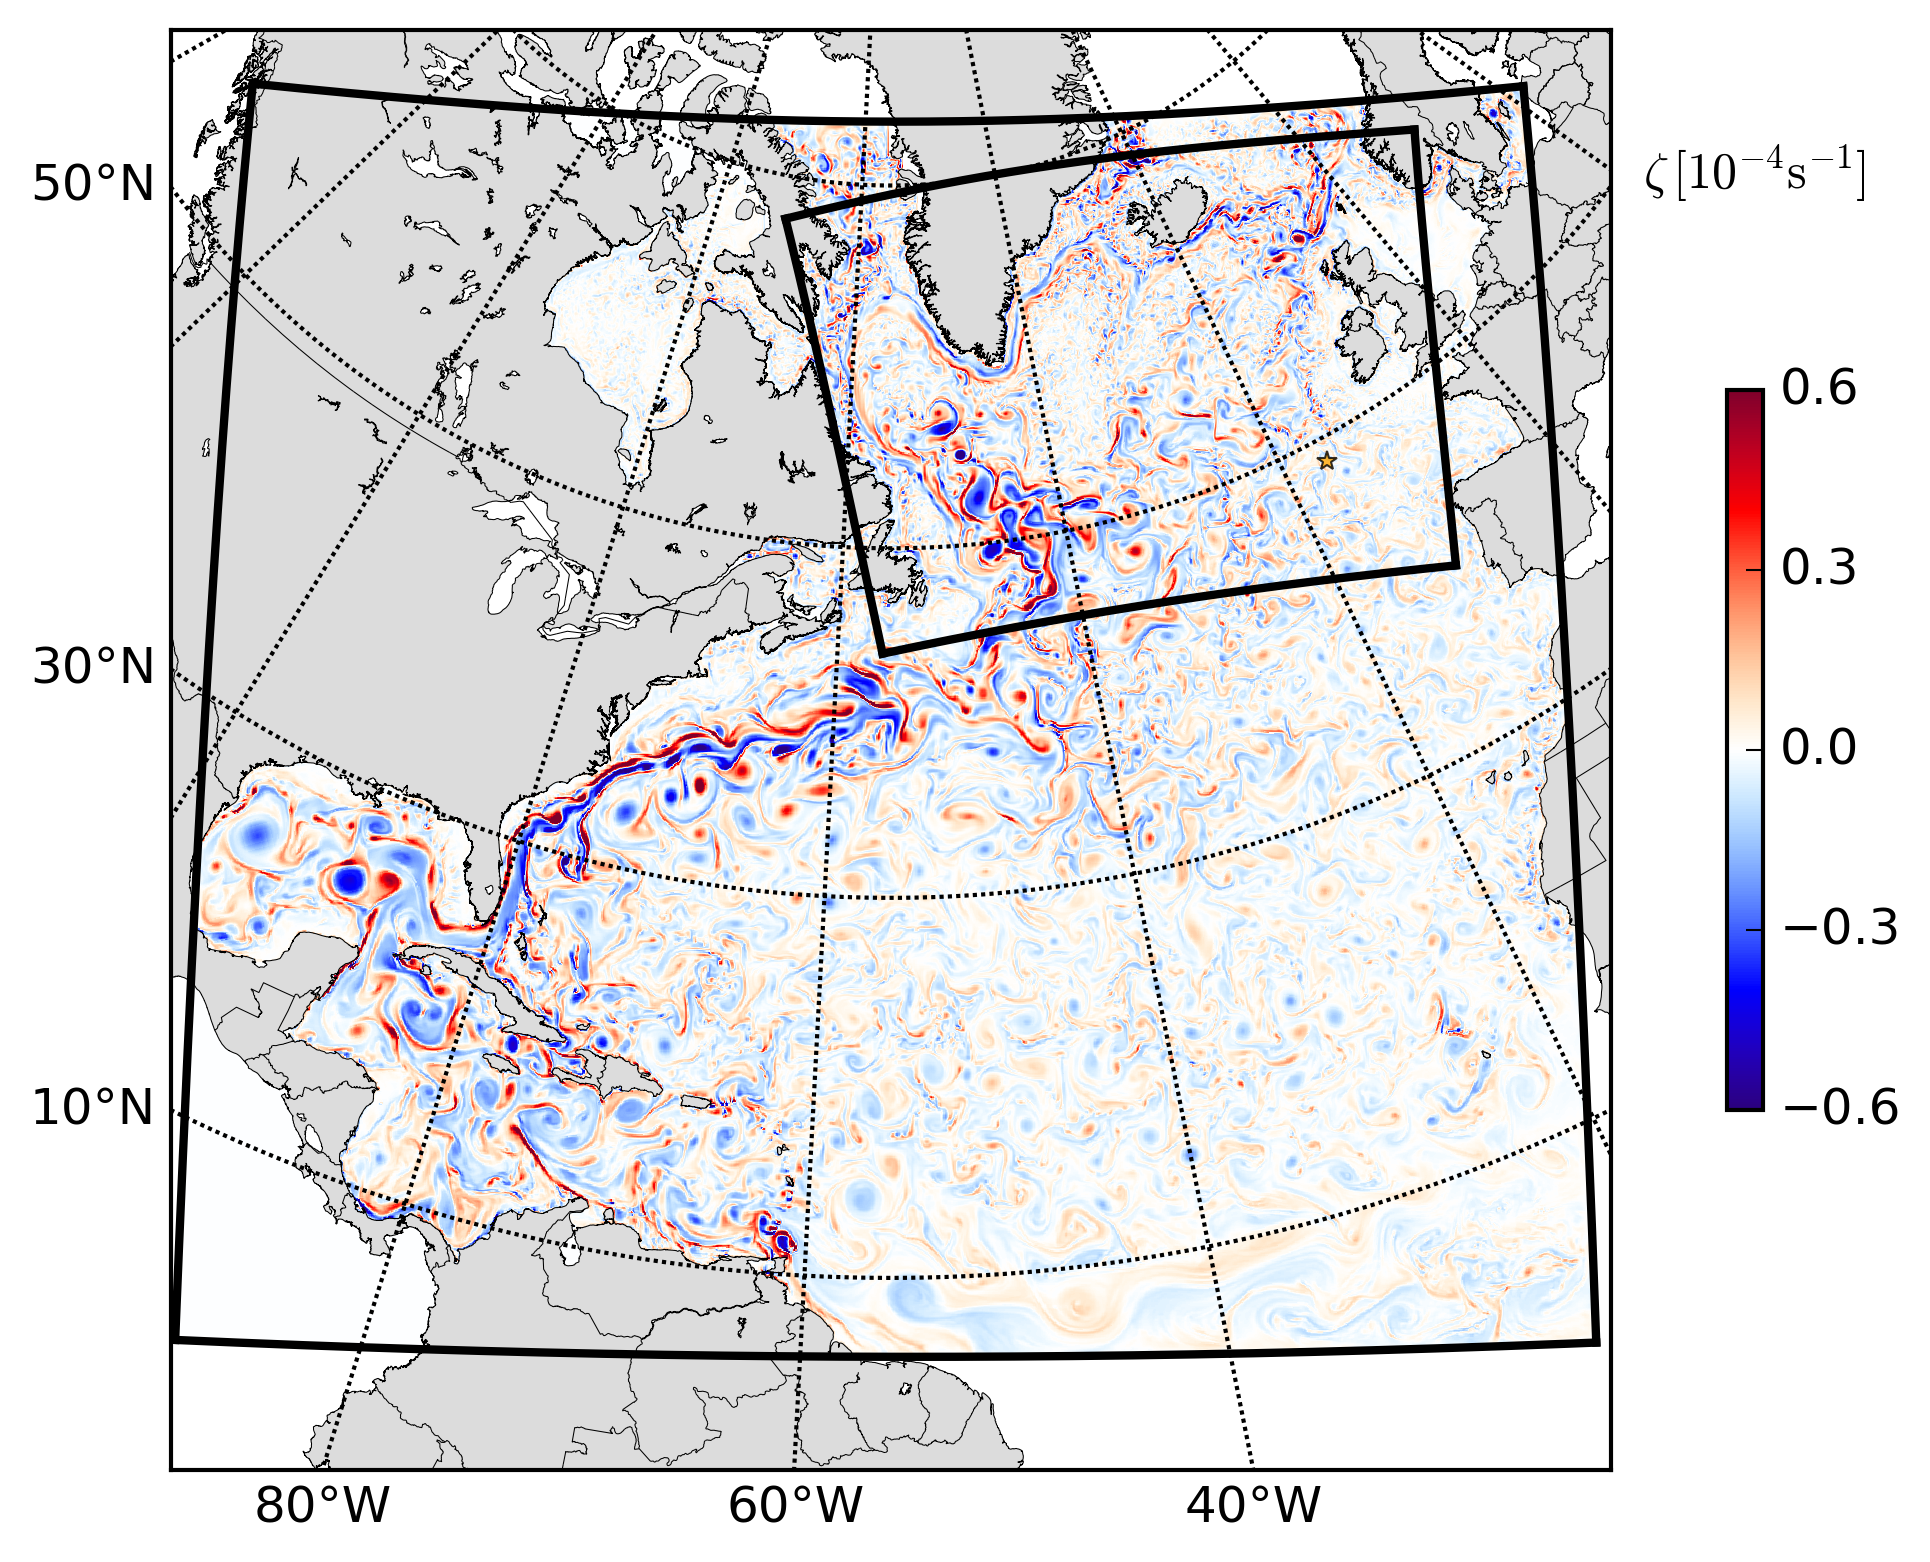
\includegraphics[width=10cm]{./fig/vrt500_and_nest.png}}
\caption{Snapshot of the relative vorticity at 500 m depth in the North Atlantic. The parent grid ($\Delta x \approx 6$ km) covers most the North atlantic, and the child grid ($\Delta x \approx 2$ km) covers the subpolar gyre.}
\label{domain}
\end{figure} 

Bathymetry for both domains is constructed from the SRTM30 PLUS dataset (available online at \url{http://topex.ucsd.edu/WWW_html/srtm30_plus.html}) based on the 1 min \citep{sandwell1997} global dataset and higher resolution data where available. A Gaussian smoothing kernel with a width 4 times the topographic grid spacing is used to avoid aliasing whenever the topographic data are available at higher resolution than the computational grid and to ensure the smoothness of the topography at the grid scale. Also, to avoid pressure gradient errors induced by terrain-following coordinates in shallow regions with steep bathymetric slope \citep{beckmann1993}, we apply local smoothing of the bottom topography where the steepness of the topography exceeds a factor r=0.2. 


Initial and horizontal boundary data for the largest domain are taken from the Simple Ocean Data Assimilation (SODA, \citet{carton2008}). The simulation is run from January 1st, 1999 to December 31st, 2010. It is spun up for 3 years, and the following 8 years are used to generate boundary conditions for the child grid. The surface forcings are daily ERA-INTERIM data for the parent grid and 12-hourly ERA-INTERIM data for the child grid. A weak salinity correction flux is used at the surface of the domain toward the ISAS13 climatology \citep{gaillard2016} to account for missing freshwater fluxes in the western part of the domain.


The North Atlantic and subpolar gyre simulations have 50 and 80 vertical levels, respectively. Vertical levels are stretched at the surface and bottom \citep{lemarie2012} to have a better representation of the surface layer dynamics at the top and flow-topography interactions at the bottom. The depth of the transition between flat z levels and terrain-following $\sigma$ levels is $h_{cline} = 300$ m. The two parameters controlling the bottom and surface refinement of the grid are $\sigma _b=2$, $\sigma _s=7$ for the parent grid and $\sigma _b=3$, $\sigma _s=6$ for the child grid. The vertical mixing of tracers and momentum is done by a k-$\epsilon$ model (GLS, \citet{umlauf2003}). The effect of bottom friction is parameterized through a logarithmic law of the wall with a roughness length $Z_{0} = 0.01$ m.

\section{Mean Currents and variability}
\subsection{Mean circulation}


We want to investigate what is driving the SPG dynamics in an eddy resolving model, so we first need to validate the mean circulation in our simulations. Mean velocities from the two simulations (NATL and POLGYR) at the surface and averaged between 1000 and 1500-m are shown in figure \ref{vel}. We present at the bottom of figure \ref{vel} the amplitudes of the current from the ANDRO database at the surface and averaged between 1000 and 1500-m depth \citep{ollitrault2013,lebedev2007}. The ANDRO data has been binned on a $0.5^{\circ}\times 0.5^{\circ}$ grid where cells with less than 10 data points have been removed. 

The NAC represents a boundary between the Subtropical and the Subpolar gyres, and oceanic models tend to have difficulties in reproducing its dynamics and particularly its  Northern extension known as the NorthWest Corner (NWC) \citep{bryan2007,hecht2008,drews2015}. As shown by \citet{wang2017} the dynamics in this area is driven by a combine effect of the advective term and of the JEBAR \citep{mertz1992}, meaning that both horizontal resolution and the topography are important in representing this feature. Its Northward extension centered at 50$^{\circ}$ N, 48 $^{\circ}$ W \citep{lazier1994} is coherent with our simulations, which limits the apparition of the so called "cold-bias" that can play a role in the low frequency variability \citep{drews2017}. After turning westward the tree branches of the NAC, being constrained by topography \citep{bower2008}, cross the Mid Atlantic Ridge (MAR) in three deep fracture zones: the Charlie-Gibbs Fracture Zone (CGFZ, 52.5 $^{\circ}$ N), the Faraday Fracture Zone (FFZ, 50$^{\circ}$ N) and the Maxwell Fracture Zone (MFZ, 48$^{\circ}$ N) \citep{bower2002}. In observations, the Northern branch of the NAC passing through the CGFZ is more intense and corresponds to the main pathway across the MAR. The three branches are well represented in the simulations with, at the surface, an overestimation of the Southern branch and an underestimation of the Northern branch. The circulation in POLGYR is closer to the observations with a better representation of the flow at the CGFZ even if the amplitude is still slitghly underestimated. 

After crossing the MAR, the three branches head North with the two Northern one feeding the interior of the Iceland basin and Rockall Plateau, while the water coming from the MFZ, that did not recirculate Southward, is flowing through the Rockall Trought (RT) \citep{daniault2016}. Most of the models tend to be consistent for the circulation in the Eastern Basin \citep{treguier2005,deshayes2007} with a good positioning of the two main branches passing respectively in the Maury channel (deepest part of the Iceland Basin west of Hatton Bank) and the RT. In NATL, the RT branch is too intense compared to ANDRO and there is a strong Southward flow at depth in the western part of the RT due to the wrong representation of the Faroe Bank channel. As the topography is strongly smoothed, the channel is not properly represented and does not allow all the dense water coming from the Nordic Seas through the Faroe-Shetland overflow to feed the Iceland Scotland Overflow Water (ISOW) properly \citep{hansen2016,kanzow2014}. Thus, the water is recirculating in the RT and created this pattern. The problem is solved by increasing the horizontal resolution and improving the topography representation, which corresponds to a wider opening of the channel, allowing a more realistic circulation in the RT. 


While part of the flow continues to the Nordic Seas \citep{rossby2012}, the other part follows the Reykjanes Ridge. Using an eddy-resolving simulation \citet{Xu2010} showed that most of the ISOW flows from the Iceland Basin to the Irminger Basin through the Bight Fracture Zone and the CGFZ. This result is consistent with estimates of the RREX cruise 2015 \citep{petit2018}. Our Subpolar gyre intensity, computed as the cumulative transport from Iceland to 53.15$^{\circ}$N along the crest of RR, is equal to -25 Sv  and compares well with the -21.9 $\pm$ 2.5 Sv  estimate in \citet{petit2018}. 


Numerous recirculations are present in the subpolar gyre, many of them happen near the intense boundary currents along Greenland and around the Labrador sea \citep{reverdin2003, flatau2003,cuny2002}. The recirculation cells present in the Labrador sea \citep{lavender2000,cuny2002} seem to make surface and intermediate water recirculate in the Irminger basin \citep{Holliday2009}. Theses features are mainly driven by the topography and the wind as described in \citet{kase200,spall2003}, and are stable in time \citep{palter2016}. Some models are unable to reproduce correctly the recirculation cells, especially the one joining West Greenland from West Labrador \citep{treguier2005}. In our case, this recirculation is well represented with a North extension being at 60$^{\circ}$ N, which matches with the observation from \citep{lavender2005}. This counter current joins the recirculation at the tip of Greenland but, at depth, the main part of the flow seems to be redirected toward the Northern branch of North Atlantic Current, instead of being advected inside Irminger basin, creating a direct connection between the two regions.

\begin{figure}[H]
\centerline{\includegraphics[width=18cm,height=20cm]{./fig/vel_aviso_roms_andro_quiv_test.png}}
\caption{Surface velocity (left) and 1000-m velocity (right) in NATL (top), POLGYR (middle) and ANDRO (bottom). For a better comparison we marred the simulations resolution to match the $0.5^{\circ}\times0.5^{\circ}$ resolution of ANDRO}
\label{vel}
\end{figure}

\subsection{The mesoscale activity}

The mesoscale activity plays a big role in redistributing the water masses properties \citep{dejong2016,zhao2018b}. The presence of mesoscale eddies can be inferred by their signatures on the Eddy Kinetic Energy (EKE). From the surface EKE signal extracted from Argo floats on a $1^{\circ}\times1^{\circ}$ grid (Fig. \ref{energy}), we retrieve the main hot spots described by \citet{flatau2003} in the SPG: namely the Labrador Sea, the Irminger and Iceland basins. Those signals are mainly due to generation of mesoscale eddies through baroclinic and barotropic instabilities of the boundary currents.

EKE amplitudes in the model are smaller than in observations, but the eddy activity is enhanced when the resolution of the model is increased. The POLGYR simulation and observational data display similar patterns in the Labrador and Iceland basins. The EKE maximum on the western flank of the Reykjanes Ridge (RR) present in ANDRO does not show up in NATL starts being resolved in POLGYR. 


A way to quantify the mesoscale activity at depth is to look at the vertical isopycnal displacements. When referenced to a mean, it represents the Eddy Available Potential Energy (EAPE) or the amount of energy stored in the potential energy reservoir due to mesoscale activity \cite{lorenz1955}. This quantity is a proxy of the baroclinic activity in the interior of the ocean. We compare EAPE computed from the simulations with the atlas of \citet{roullet2014} constructed from Argo data (Fig. \ref{energy}). In NATL (at 6 km resolution) most of the baroclinic activity alreadys seems well resolved. However, observations highlight an EAPE maximum on the western flank of the RR that is missing in NATL, but appears only in POLGYR (at 2 km resolution). On the contrary, strong patches of EAPE are visible along the boundary currents of the western half of the SPG in NATL, but are not visible in observations. Interestingly these patterns weaken in POLGYR, potentially pointing to a change in the vertical structure of the currents at higher resolution. Another factor to take into consideration is the lack of Argo measurements close to the boundaries, which might underestimate EAPE at these locations.



\begin{figure}[H]
\centerline{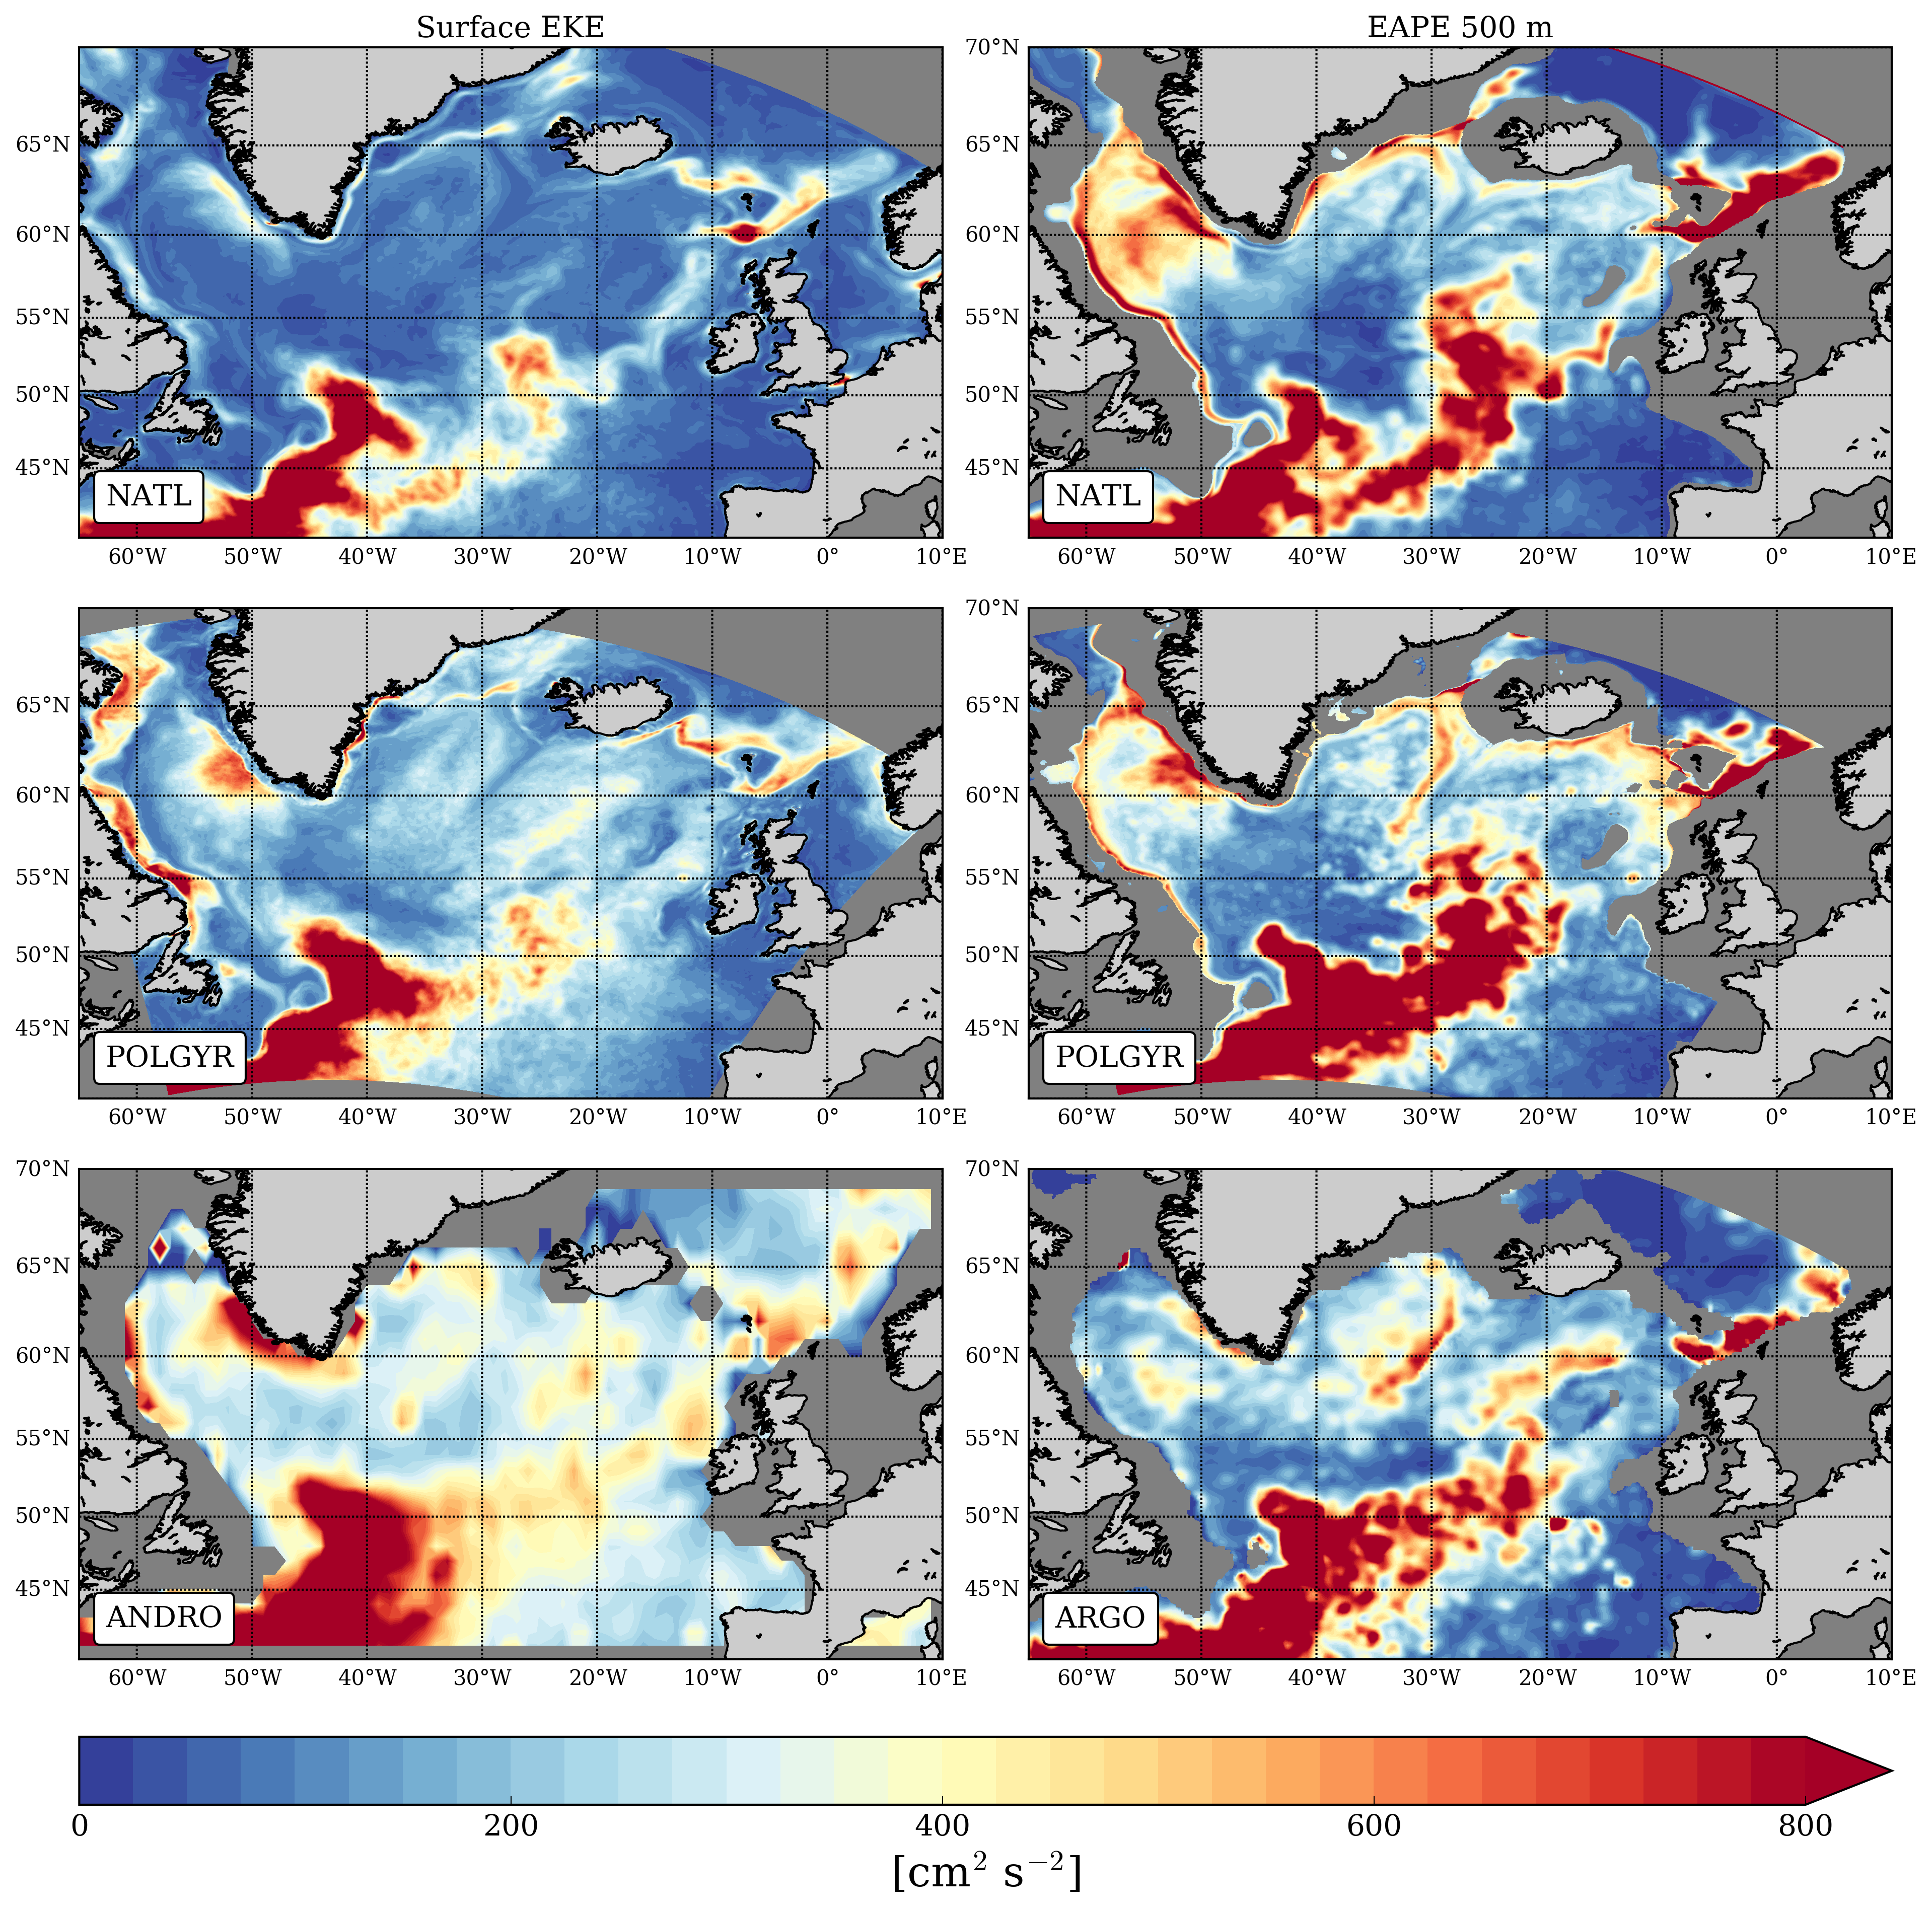
\includegraphics[width=18cm]{./fig/eke_eape_basemap_vert.png}}
\caption{Mean Surface Eddy Kinetic Energy (left) and Mean Eddy Available Potential Energy between 2002 and 2008 from the NATL (top) and POLGYR (middle) simulations. These have to be compared with mean EKE from the Andro database (lower left) and the mean EAPE from the Atlas of \citet{roullet2014} (lower right)}
\label{energy}
\end{figure}



\section{On the dynamics of the North Atlantique Subpolar gyre }

\subsection{An overall view of the subpolar gyre vorticity balance}

To study the dynamics of the gyre we choose to compute the barotropic vorticity balance. The barotropic vorticity equation is obtained by integrating the momentum equations in the vertical and cross-differentiating them \citep{gula2015}:

$$\underbrace{\frac{\partial \Omega}{\partial t}}_{rate} = -\underbrace{\nabla.(f\overline{u})}_{planet.vort.adv}+\underbrace{\frac{J(P_b,h)}{\rho _0}}_{bot.pres.torque} +\underbrace{k.\nabla \times \frac{\tau _{wind}}{\rho_{0}}}_{wind.curl} -\underbrace{k.\nabla \times \frac{\tau _{bot}}{\rho_{0}}}_{bot.drag.curl} +\underbrace{D_{\Sigma}}_{horiz.diffusion}-\underbrace{A_{\Sigma}}_{NL advection}$$,

where the vorticity is the curl of the vertically integrated component of the velocity between the bottom and the surface. It is possible to decompose $-\nabla.(f\overline{u})=-\beta \overline{V}-f \frac{\partial \eta}{\partial t}$. As we take the mean on a long time period $\frac{\partial \eta}{\partial t} \approx 0$ we write  $-\nabla.(f\overline{u})= - \beta \overline{V}$

The non linear term can be written as:

$$A_{\Sigma}= \frac{\partial ^2 (\overline{vv}-\overline{uu})}{\partial x \partial y}+\frac{\partial ^2 \overline{uv}}{\partial x \partial x} -\frac{\partial ^2 \overline{uv}}{\partial y \partial y}$$

where (u,v) denote the horizontal components of the flow in (x,y) directions and the overbar defines a vertically integrated quantity:

$$\overline{u}=\int^{\eta}_{-h} u dz$$

with $\eta(x,y,t)$ the free surface height and $h(x,y)$ the topography. 

The bottom pressure torque J(P$_b$,h) is the Jacobian of the bottom pressure and the depth of the topography. It encompasses the effects of the varying topography on the flow, and is known to play a key role in the barotropic vorticity equilibrium of the subpolar gyre (fig \ref{spatial_BV}). In an idealized case of a geostrophic current flowing along a topography in free-slip condition, the BPT can be written $\frac{J(P_b,h)}{\rho _0}=f u_b.\nabla h$. Given the kinematic condition at the bottom: $-u_b . \nabla h =w_b$, the BPT can be then written $\frac{J(P_b,h)}{\rho _0}=-fw_b$, which highlight the relation between the BPT and vortex stretching when the flow crosses an isobath.

\begin{figure}[H]
\centerline{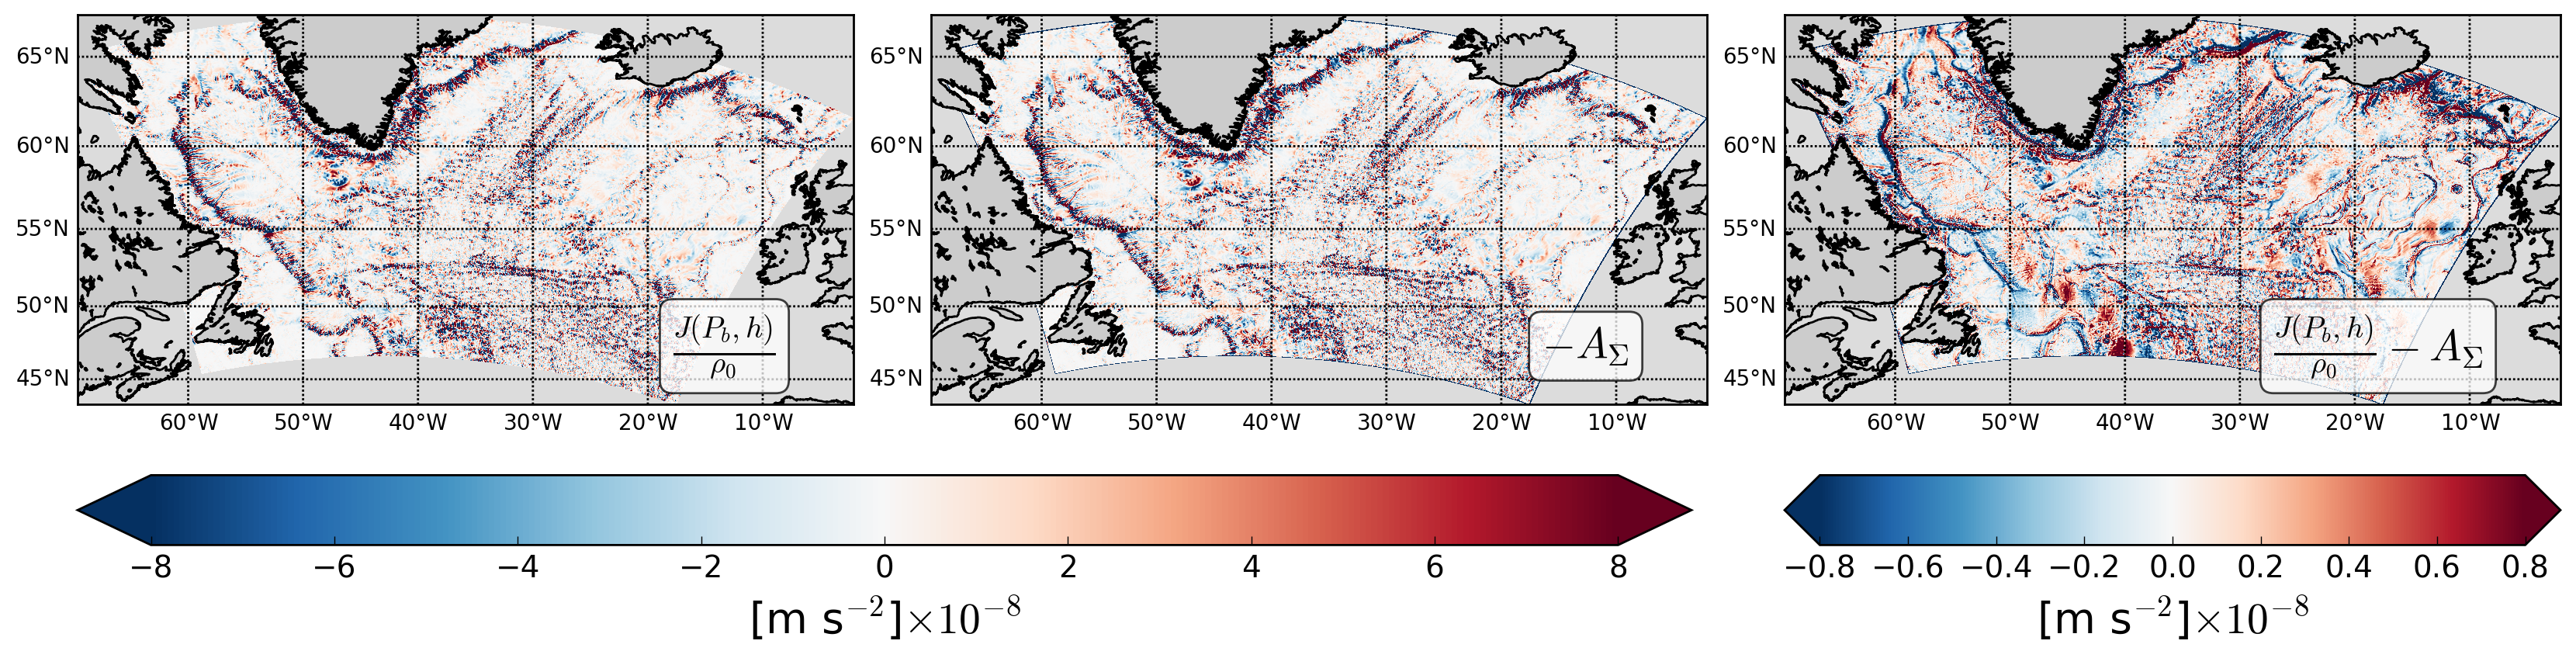
\includegraphics[width=20cm]{./v_b/BPT_NL_sum.png}}
\caption{Time mean (a) bottom pressure torque, (b) non-linear terms, and (c) sum of the two for the 2-km North Atlantic subpolar gyre simulation.}
\label{BPT_NL_unsmoothed}
\end{figure} 

\begin{figure}[H]
\centerline{\includegraphics[width=20cm]{./v_b/BV_terms_gyre_smooth_vert.png}}
\caption{Mean barotropic vorticity terms in the North Atlantic subpolar gyre horizontally smoothed with a kernel of $1^{\circ}$ radius}
\label{spatial_BV}
\end{figure} 

The barotropic vorticity terms have already been computed for the North Atlantic using different models (OCCAM, ECCO, UVic ESCM, POP) at different resolutions ($1.8^{\circ}\times3.6^{\circ}$, $1^{\circ}$, $0.25^{\circ}$, $0.2^{\circ}\times 0.4^{\circ}$ $0.1^{\circ}$) in \citet{hughes2001}, \citet{spence2012}, \citet{sonnewald2019}, and \citet{yeager2015}. Their major result is that the barotropic vorticity balance in the subtropical and subpolar gyres is at first order a balance between $\beta$V, $\nabla \times \frac{\tau _{wind}}{\rho_{0}}$ and $\frac{J(P_b,h)}{\rho _0}$. 

In the subtropical gyre, the barotropic vorticity balance is close to a Sverdrup balance away from the boundaries ($\beta V \approx \nabla \times \frac{\tau _{wind}}{\rho_{0}}$), while the closure of the northward branch of the gyre at the western boundary is done primarily through BPT ($\beta V \approx \frac{J(P_b,h)}{\rho _0}$)  \citep{schoonover2016}.

The barotropic vorticity balance in the SPG is slightly more complex due to the stronger impact of the topography. Along the northern and western boundaries of the SPG, the first order balance is between meridional advection and BPT ($\beta V \approx \frac{J(P_b,h)}{\rho _0}$) (\textit{e.g.} \citet{hughes2001}, their Fig. 4; \citet{yeager2015}, their Fig. 1; ), with a significant impact of the wind only in the norther part of the gyre along the Greenland coast. When the resolution of the model is increased from $1^{\circ}$ to $0.1^{\circ}$ in \citet{yeager2015}, the main balances stay qualitatively similar, showing a modest effect of the eddies. The non linear term increases mostly in the Gulf Stream and NAC regions, where it can be associated to increased meandering of the Gulf Stream and NAC. The viscous torque decreases in the boundary currents due to the lower viscosity of the model.

\subsection{Local barotropic vorticity balances in a eddying subpolar gyre}


In our simulations, the resolution increase induces much stronger qualitative differences in the local vorticity balance as the BPT now balances the advection of vorticity at leading order everywhere in the domain (Fig. \ref{BPT_NL_unsmoothed}). This is similar to the results of \citet{gula2015} in the Gulf Stream region with the same ocean model and a similar horizontal resolution. This translates the fact that the bottom pressure anomaly balances the advection term in the momentum equation as the flow attempts to follow isobaths. Both terms then exhibit small scales related to isobaths features, but with a high degree of cancellation between each other. The sum of the BPT and NL terms (Fig. \ref{BPT_NL_unsmoothed}c) is often an order of magnitude smaller than the amplitude of the terms considered individually  and exhibits patterns and amplitudes matching the advection of planetary vorticity.


Another way to get rid of the small topographic scales is to smooth all fields with a large enough length scale. NL terms in particular are expected to be smoothed out on scales larger than 1-2$^{\circ}$ \citep{hughes2001}. Fig. \ref{spatial_BV} shows all terms smoothed with a gaussian kernel of 1$^{\circ}$ radius. Even with such smoothing, the BPT and NL terms are still significantly larger than the corresponding results from the $0.1^{\circ}$ simulation of \citet{yeager2015}. However, their sum $\frac{J(P_b,h)}{\rho _0}-A_{\Sigma}$ is of the same order of magnitude than the $\beta$V and Bottom Drag Curl (BDC).

The curl of the wind stress has the same pattern and amplitude compared to \citet{yeager2015}. It is mostly positive with the strongest signal on the Eastern coast of Greenland. The amplitude of the $\beta$V term is slightly stronger than in the lower resolution simulations. In the simulations of \citet{hughes2001} and \citet{yeager2015}, the patterns of the $\beta$V term showed that the currents were much wider, reaching the interior of the gyre. Here, the patterns shows the presence of thinner and more intense currents, closely following the continental slopes.

In our simulations, the amplitude of the diffusion term due to viscosity effect ($D_{\Sigma}$) is very small, while the amplitude of the BDC is comparable to the $\beta V$. This is opposite to the results of \citet{yeager2015}. The viscous term in the $0.1^{\circ}$ POP simulation of \citet{yeager2015} is qualitatively similar in pattern  to the bottom drag curl in our simulation. The boundary conditions near the topography are quite different in the two models due to the different vertical coordinates. The z-levels coordinates have vertical walls between each level, which induce lateral viscosity and explain the pattern in \citet{yeager2015}, while the $\sigma$-levels coordinates have no lateral boundary conditions and dissipation is only due to the parameterized bottom drag. 

The amplitude of the BDC is however stronger in our simulation than the viscous term in \citet{yeager2015} and seems to play a important role in balancing the BPT and $\beta V$ terms over the shelf and on the upper part of the continental slope on the northern and western boundaries of the gyre (Fig. \ref{BDC}).

\begin{figure}[H]
\centerline{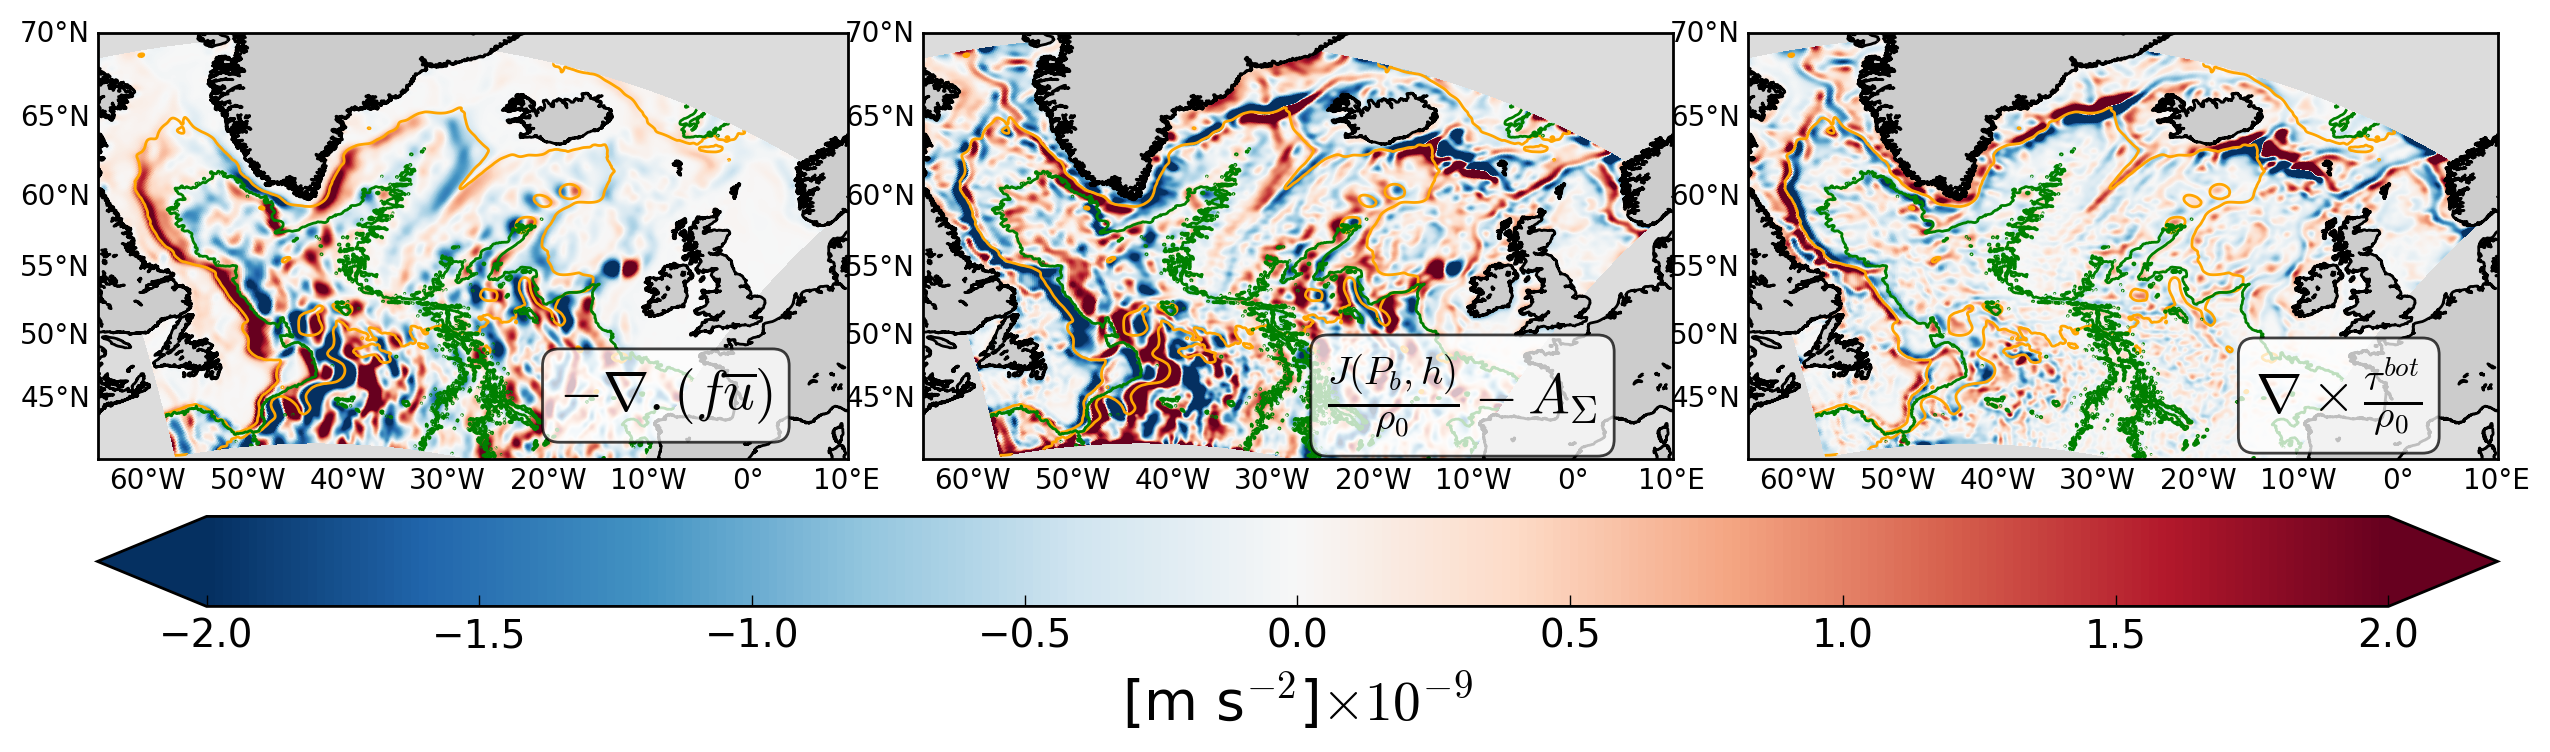
\includegraphics[width=20cm]{./v_b/BV_terms_test.png}}
\caption{Time mean (a) advection of planetary vorticity, (b) $\frac{J(P_b,h)}{\rho _0}-A_{\Sigma}$, and (c) bottom drag curl for the 2-km North Atlantic subpolar gyre simulation.}
\label{BDC}
\end{figure} 


\subsection{Barotropic nature of the currents}

As explained previously, the bottom pressure torque J(P$_b$,h) can be identified with a bottom vortex stretching term: $\frac{J(P_b,h)}{\rho _0}=f u_{gb}.\nabla h = -f w_{gb}$, where $u_{gb}$ is the horizontal geostrophic bottom flow. 

The computation of the BPT in \citet{spence2012} is even performed by directly estimating the term  $-f w_{b}$, where $w_{b}$ is the vertical velocity through the top of grid cells located directly above the seafloor. However this estimation does not take into account the ageostrophic component of the velocity at the bottom, in particular the Ekman component of the velocity due to the bottom drag. The same computation in our model leads to the results of Fig. \ref{decomp_bpt}b, which are very different from the actual bottom pressure torque \ref{decomp_bpt}a. It gives results quite similar to \citet{spence2012} with positive signals - implying downwelling of bottom currents - over most of the boundaries of the gyre. But this downwelling is a result of the Ekman currents oriented to the left of the main bottom geostrophic currents, which are flowing with the shallower topography on their right around the gyre.


\begin{figure}[H]
\centerline{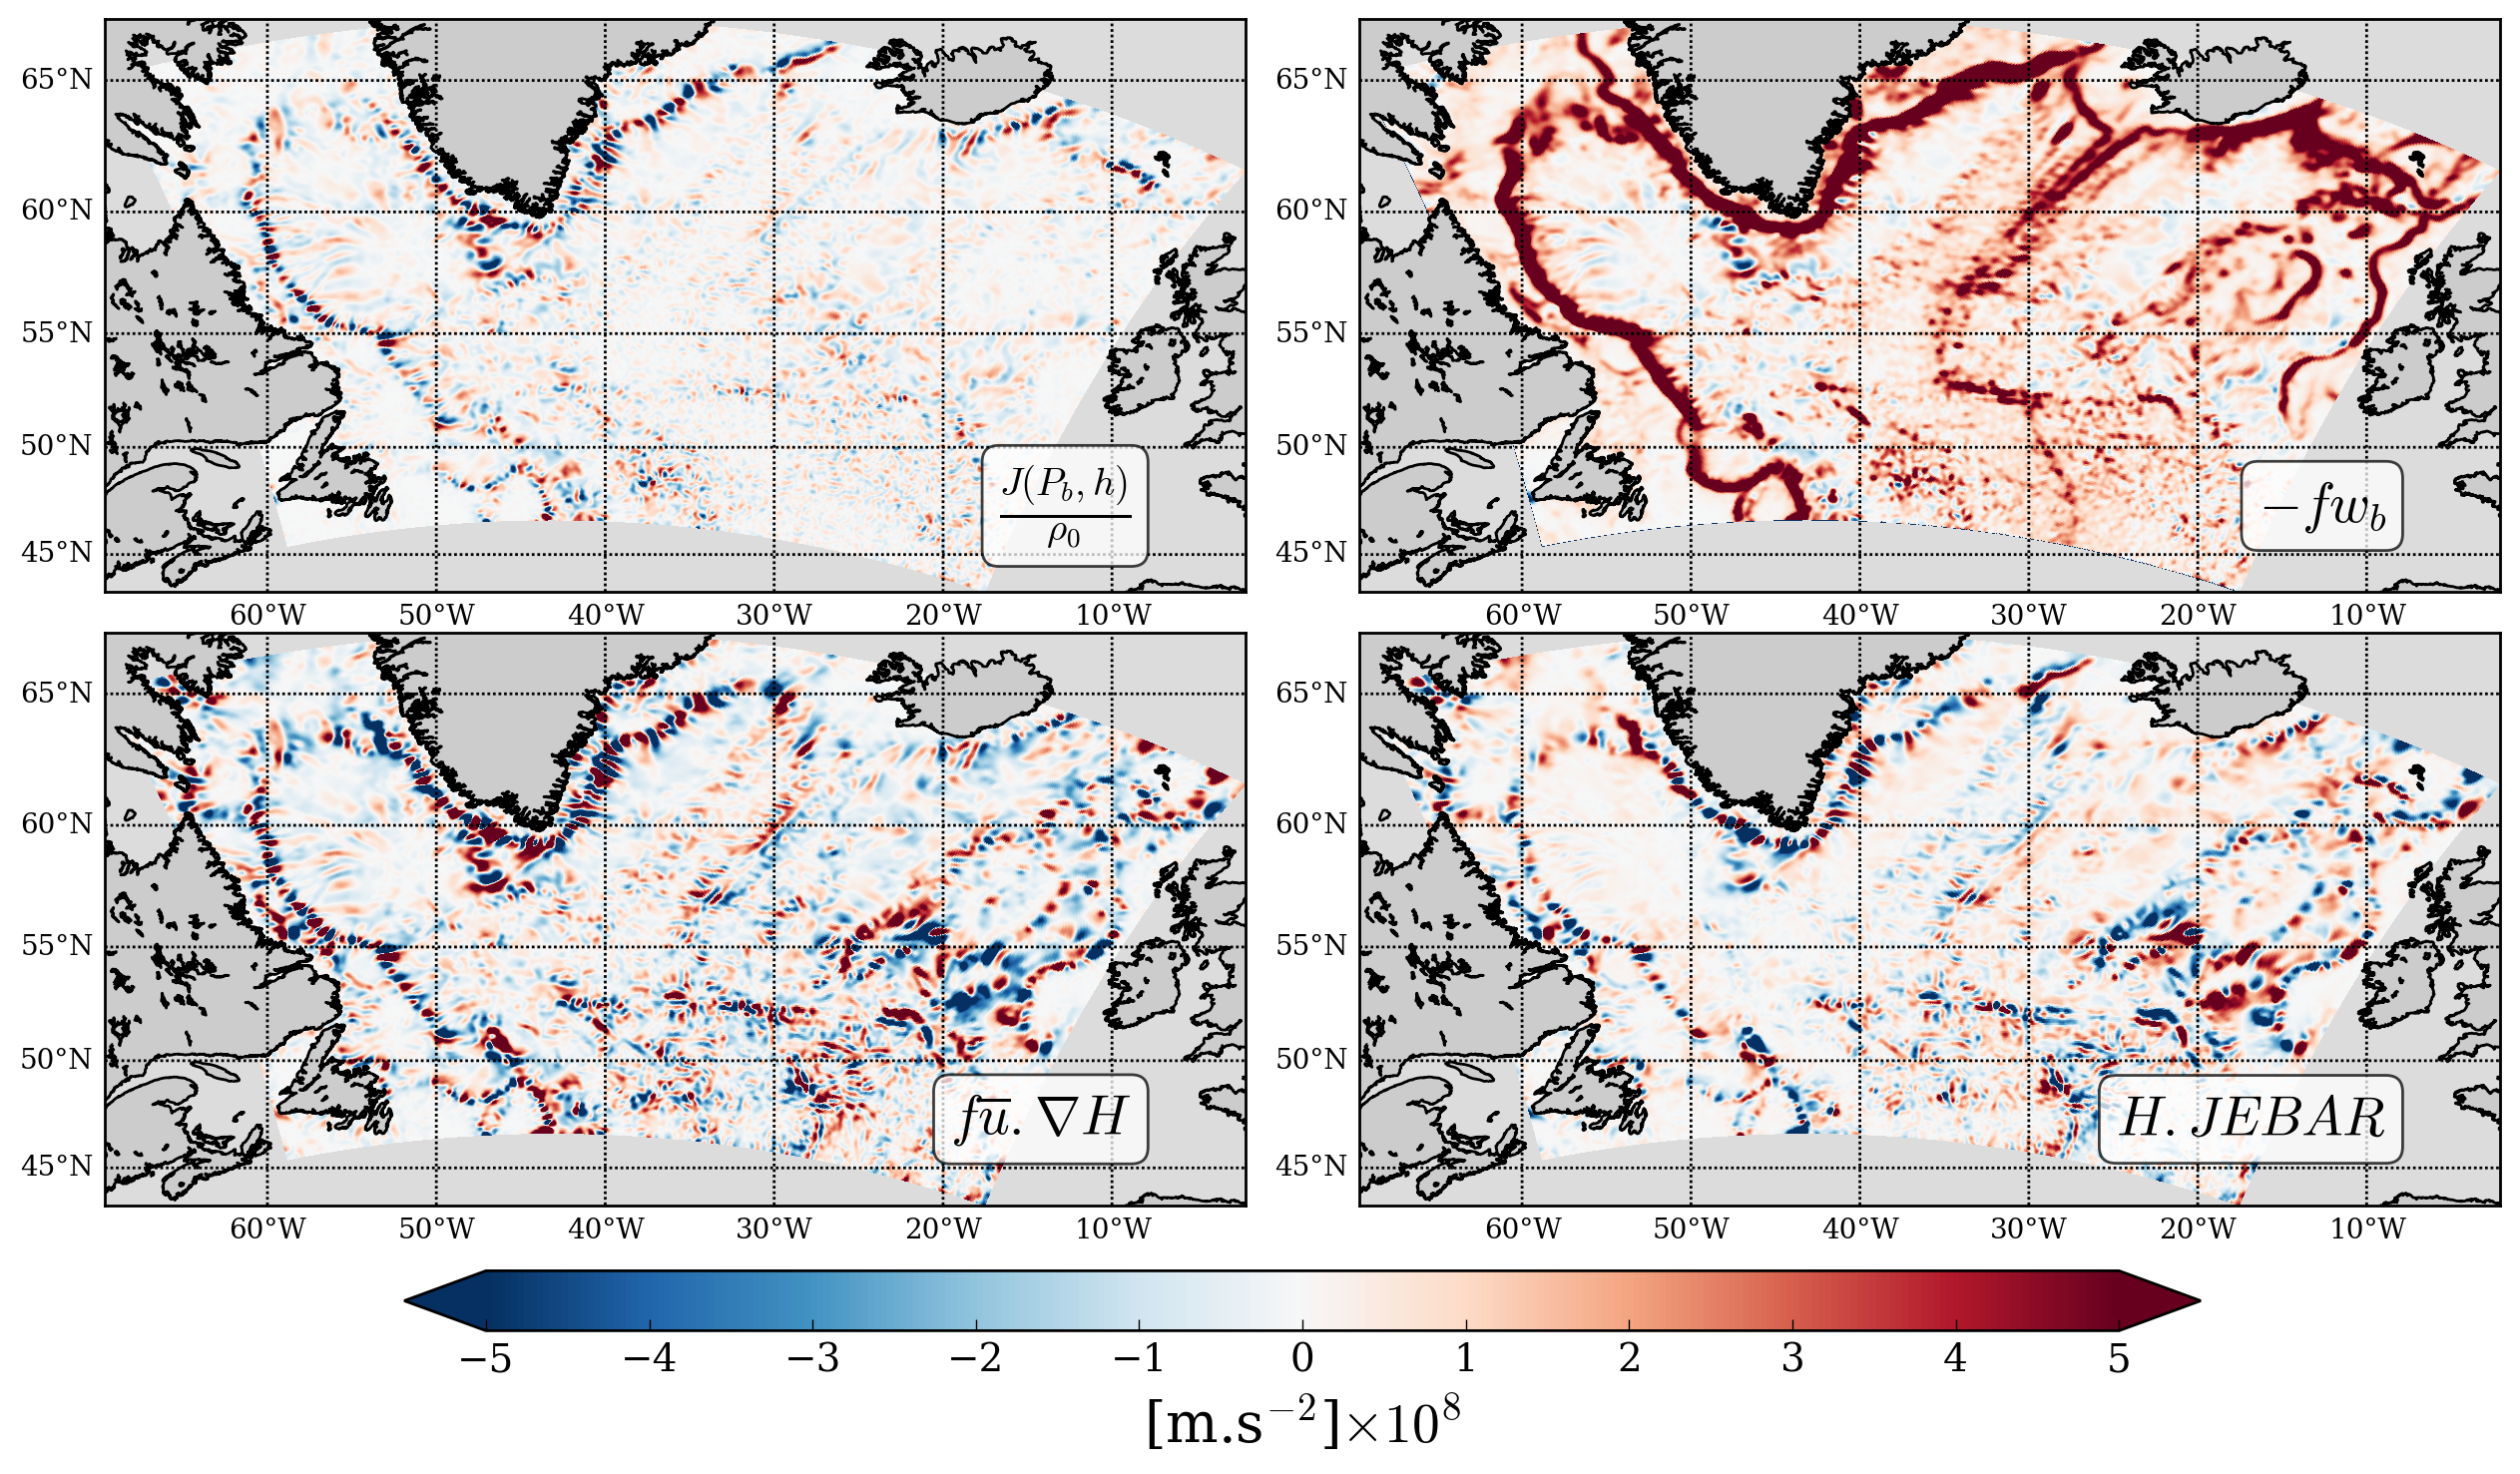
\includegraphics[width=20cm]{./v_b/decomp_bpt.png}}
\caption{Time mean (a) bottom pressure torque, (b) $-f w_{b}$, (c) $ \frac{f}{h} \overline{u} \cdot \nabla H$, and (d) $H(JEBAR)$ for the 2-km North Atlantic subpolar gyre simulation.}
\label{decomp_bpt}
\end{figure} 

Following \citet{mertz1992,yeager2015}, the BPT can be further decomposed into:

$$\frac{J(P_b,h)}{\rho _0}=f u_{gb}.\nabla h = \frac{f}{h} \overline{u_g}.\nabla h +  h(JEBAR)$$,

which illustrates that the bottom geostrophic currents that appears in the expression for BPT are the sum of a vertically averaged part and a baroclinic part directly related to the JEBAR term. The term $ \frac{f}{h} \overline{u} \cdot \nabla H$ highlights regions where the depth-averaged flow is crossing isobaths, and the $h(JEBAR)$ term where the baroclinic effects are playing a role to decouple the bottom flows from the barotropic flow through the geostrophic shear.

Along the continental slopes, on the western and northern part of the gyre, the flow is close to barotropic and the $ \frac{f}{h} \overline{u} \cdot \nabla H$ term has similar patterns and amplitudes than the BPT. This contrasts with results from \citet{yeager2015}, who found that the $h(JEBAR)$ term was almost an order of magnitude larger than the BPT in these regions. However over the southern and eastern part of the gyre, it is clear that the structure of the flow is much more baroclinic and the $ \frac{f}{h} \overline{u} \cdot \nabla H$ and  $h(JEBAR)$ terms are both an order of magnitude larger than the BPT.

\subsection{Gyre integrated barotropic vorticity balances}

The maps of the barotropic vorticity terms, with various degree of smoothing, can help identify the locally dominant terms, but do not enable us to identify the important balances at the gyre scale. Spatial integrations are performed inside the gyre (fig \ref{intgyre_BV}) to better understand the main contributors to the circulation of the subpolar gyre. 

%Using oxygen isotope \citet{chapman1986,chapman1989} shown there is a connection from West Greenland toward the Mid-Atlantic Bight (North of Cap Hatteras) by a shelf current. This alongshelf flow is independant of the mean wind and is buoyancy driven \citep{csanady1978}. The subpolar gyre seems to act as a boundary that isolated the shelf and making it independant from its circulation. 

\begin{figure}[H]
\centerline{\includegraphics[width=20cm]{./v_b/BV_int_0_diff_3.png}}
\caption{Integration of the barotropic vorticity terms over the 0 Sv contour (left) and the -3 Sv contour (right) and the difference between the two (middle)}
\label{intgyre_BV}
\end{figure} 

We perform integration of the barotropic vorticity equation in the subpolar gyre inside two different contours: the 0 Sv and the -3 Sv contours (fig \ref{intgyre_BV}). We can check that the term $\beta$V integrates to zero as we choose closed contours. The 0 Sv contour tends to overlap the upper slope and the shelf (especially along West Greenland and East Canada) while the -3 Sv contour does not take include the shelves. The main balance between the integrated terms is quite different depending of the chosen contour.

When integrated inside the -3 Sv contour (which means excluding the shelf area, Fig. \ref{intgyre_BV}c), the main sources for the cyclonic circulation of the gyre are the wind and the BPT. They are balanced by the BDC. The input of the wind does not contribute much locally, but becomes significant when spatially integrated over the gyre. The BPT is the major source of positive vorticity and helps the flow moves cyclonically around the gyre. The major sinks of vorticity are the NLA and the BDC. The BDC is very intense where the flow is close to a steep topography, as in the case of the Western Labrador Sea Current (WLSC) and the Western Greenland Current, but also near the CGFZ. 

When integrated inside the 0 Sv contour (Fig. \ref{intgyre_BV}a), the balance is slightly different. The wind is still a major contributor for the cyclonic circulation and the BDC still represents the major sink of vorticity. However, the NL term replaces the BPT as a source of cyclonic vorticity for the gyre. In this interpretation, both the wind and the NL term forces the gyre cyclonically, while the drag balances this input along steep topography. 

The difference between the two balances is highlighted by looking at the balance in the region in-between the 0 Sv and the - 3 Sv contours, which covers the upper slope and the shelf. It corresponds to a balance between BPT, NLA and bottom drag. This balance is close to the one describe in \citet{csanady1978} and evokes a buoyancy driven flow in this area. This result seems to be coherent with previous work with a different dynamic in shallow water. %Following the idea of Chapman 86-89 were the shelf does not interact with the subpolar gyre, it feels natural to exclude the upper slope and the shelf from our study. To do so in the following we will focus on the -3 Sv contour which is the biggest close domain excluding the boundary.
 
\subsection{Barotropic vorticity balance in the interior of the gyre}

It is clear from the patterns of the different terms of the barotropic vorticity balance that the local balances over the boundary currents are very different than what is happening in the interior of the gyre. The classical picture of a gyre interior in a quasi-Sverdrup balance that applies in the sutropical gyre,  does not seem to apply here. 

To better understand what drives the interior of the subpolar gyre, we further divide the domain into an inner part and a boundary part, as represented in fig. \ref{int_bound_inner_BV}. The two domains are defined using the -3 Sv line as previously, and the 3000 m isobath. What is between the -3 Sv line and the 3000m isobath is considered as the boundary zone and the rest is considered as the inner zone. The choice of the 3000 isobath is purely subjective but the results are not sensitive to the choice of the isobath. 

\begin{figure}[H]
\centerline{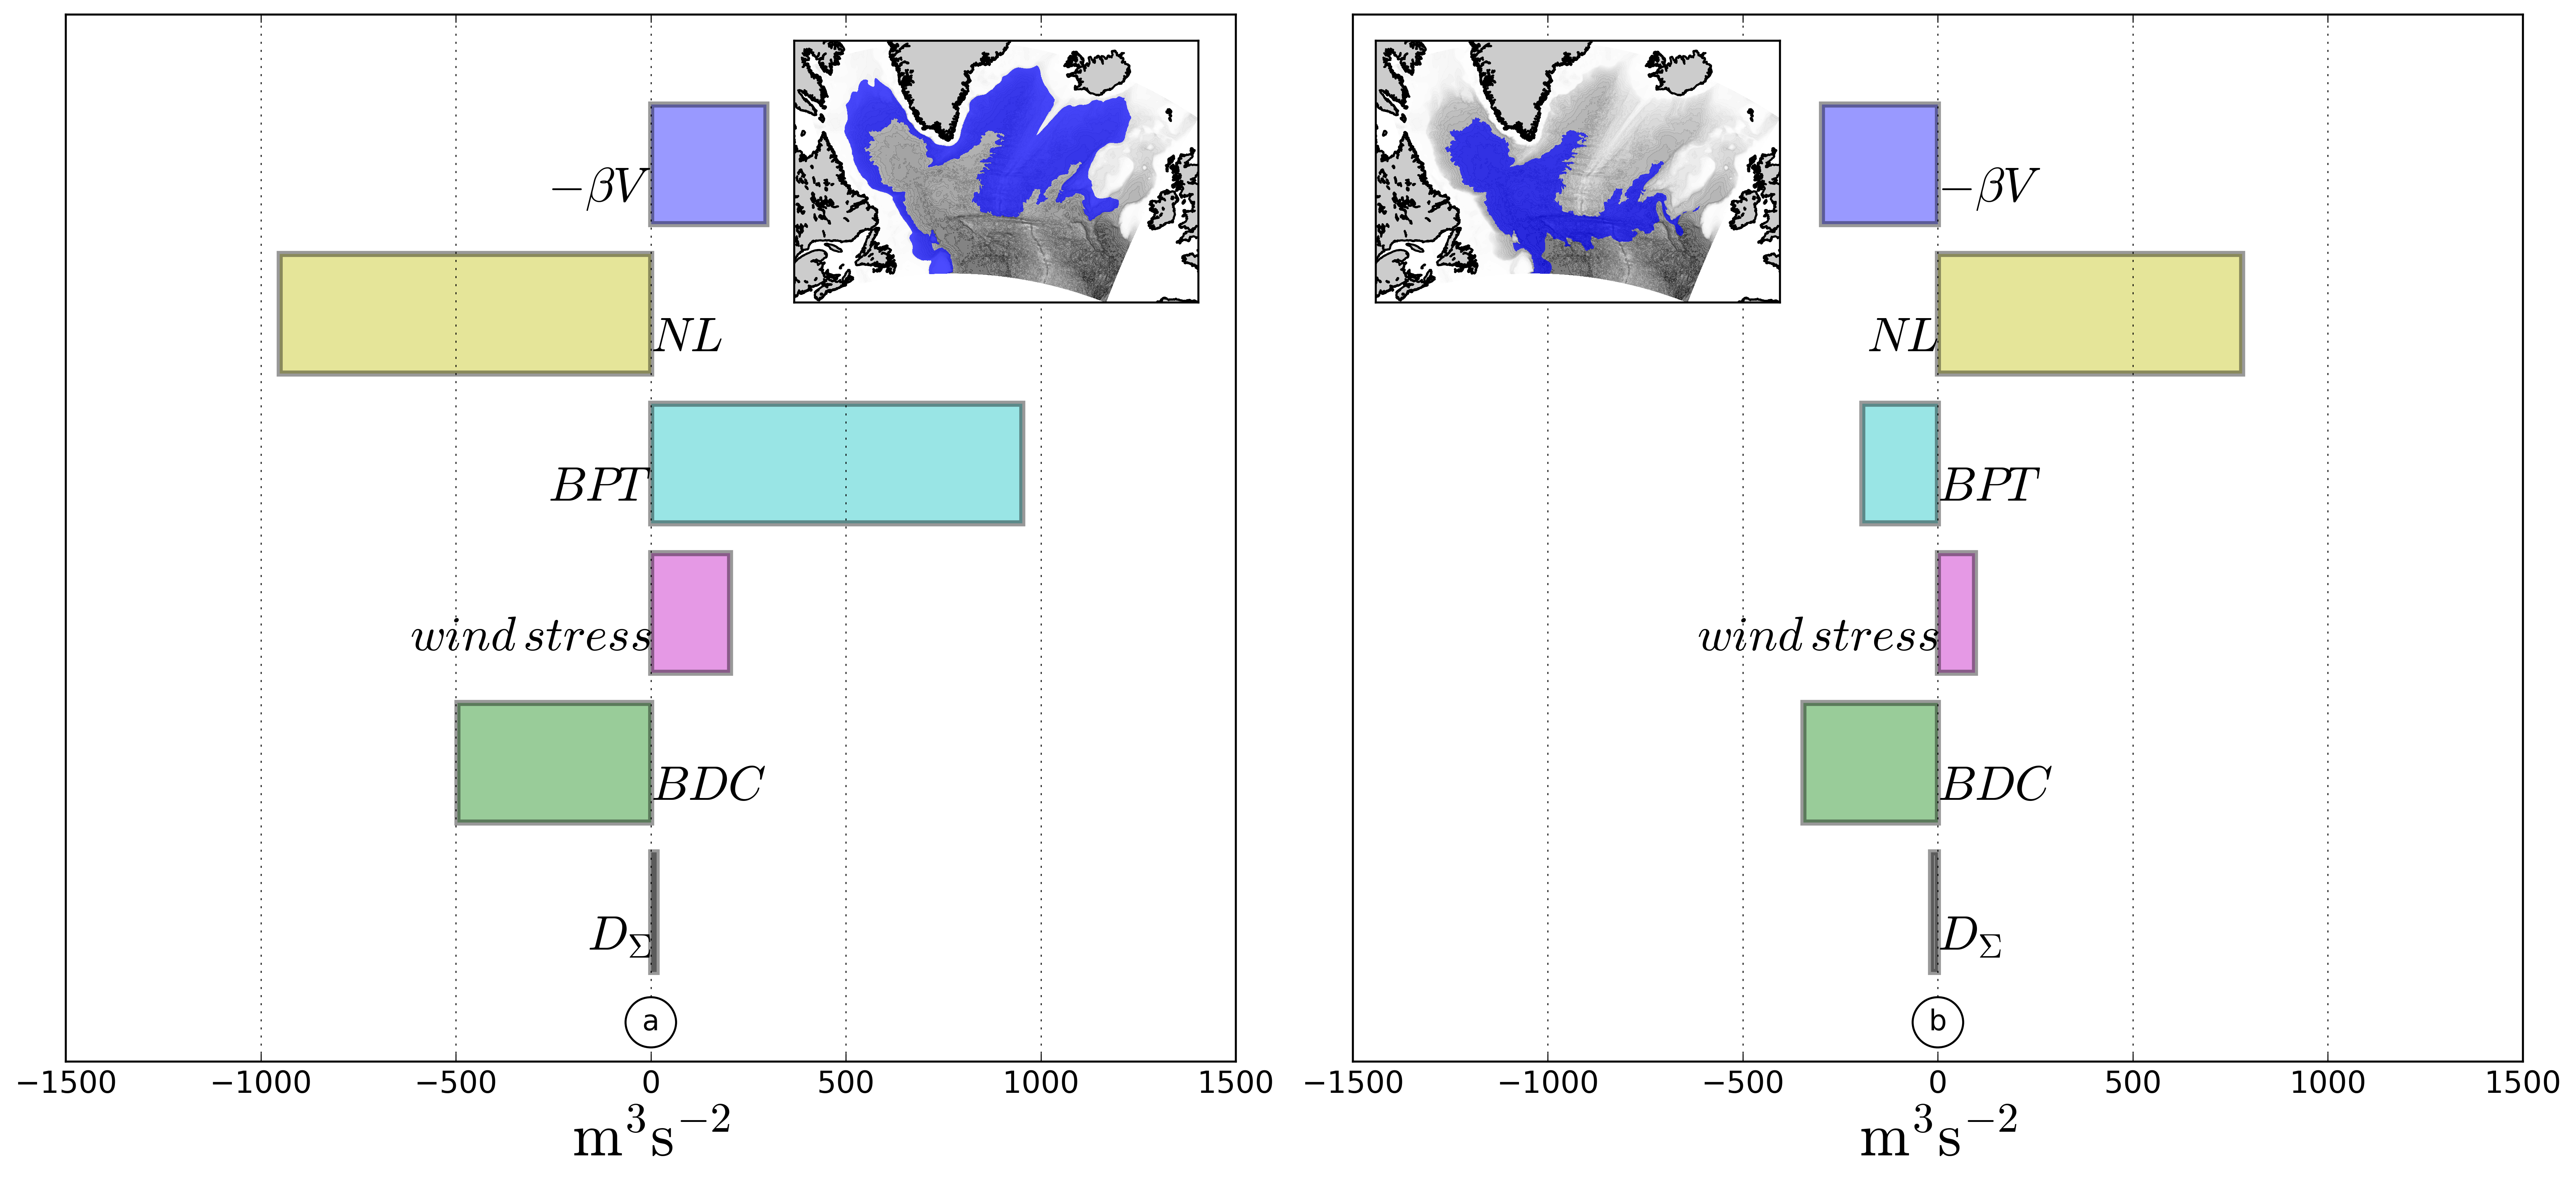
\includegraphics[width=15cm]{./v_b/BV_int_bound_inner_3sv.png}}
\caption{Integration of the barotropic vorticity terms in boundary and inner area for the -3 Sv contour}
\label{int_bound_inner_BV}
\end{figure} 

In the boundary zone, the main source of cyclonic vorticity is the BPT. Secondary sources are the curl of the wind and the $\beta$V. The negative NL term sign indicates vorticity advection outside of this domain toward the shelf or the inner gyre.

In the inner zone, the NLA term represents the major contribution to the cyclonic circulation. It is balanced by the BDC, the BPT and the $\beta$V terms.  Contributions from the BDC are of similar magnitude in the inner and boundary zones.  The wind input of vorticity is smaller than in the boundary zone, as the major wind source of vorticity is located along the Greenland area (fig \ref{spatial_BV}) and not uniformly distributed over the gyre. It confirms that the inner part of the gyre in not in Sverdrup balance at the first order, which would imply a dominant balance between a negative $\beta$V and a positive input from the curl of the wind stress, but is driven by nonlinear effects.


The comparison between balances in the inner and boundary zones seems to indicate that the NLA term helps to redistribute vorticity from the boundary toward the interior of the gyre. %The cyclonic vorticity is provided by the BPT at the boundaries of the gyre, and balanced by a sink of positive vorticity by the BDC all over the gyre.

\subsection{Characterisation of the Non Linear advective term}


The Non linear advective term is obtained by taking the curl of the vertically integrated momentum equation. The NL term is locally important and balances the bottom pressure torque around topographic features. When integrated over the gyre it seems to play a role in advecting the barotropic vorticity from the boundary toward the inside of the gyre. This component is quite difficult to interpret as  many processes are hidden inside the vertical and time integrals. 

By decomposing the velocity in a barotropic and baroclinic part ($u = \overline{u} + u'$) the NL advection term can be written as:

$$A_{\Sigma}=\underbrace{A(\overline{u},\overline{v})}_{A^{bt}_{\Sigma}}+\underbrace{A(u',v')}_{A^{bc}_{\Sigma}}$$

where the barotropic part can be written as $A(\overline{u},\overline{v})= \overline{u}\Omega _x +\overline{v}\Omega _y$ which is the advection of the barotropic vorticity by the barotropic flow.  

When integrated over the inner gyre (Fig. \ref{int_NL}), the contribution is evenly divided between barotropic and baroclinic contributions. The baroclinic contribution is mainly provided by the NWC. The remaining part comes mostly from the South-Eastern boundary, as the export of barotropic vorticity by the baroclinic NL term along the topography is small. In the boundary area the barotropic contribution is the dominant one. It is used to export barotropic vorticity inside the gyre.  %Considering the need from the inner part, the boundary value is too high meaning that a large quantity of the mean NL advection term only helps locally for the balance of the boundary current. The remaining part 

\begin{figure}[H]
\centerline{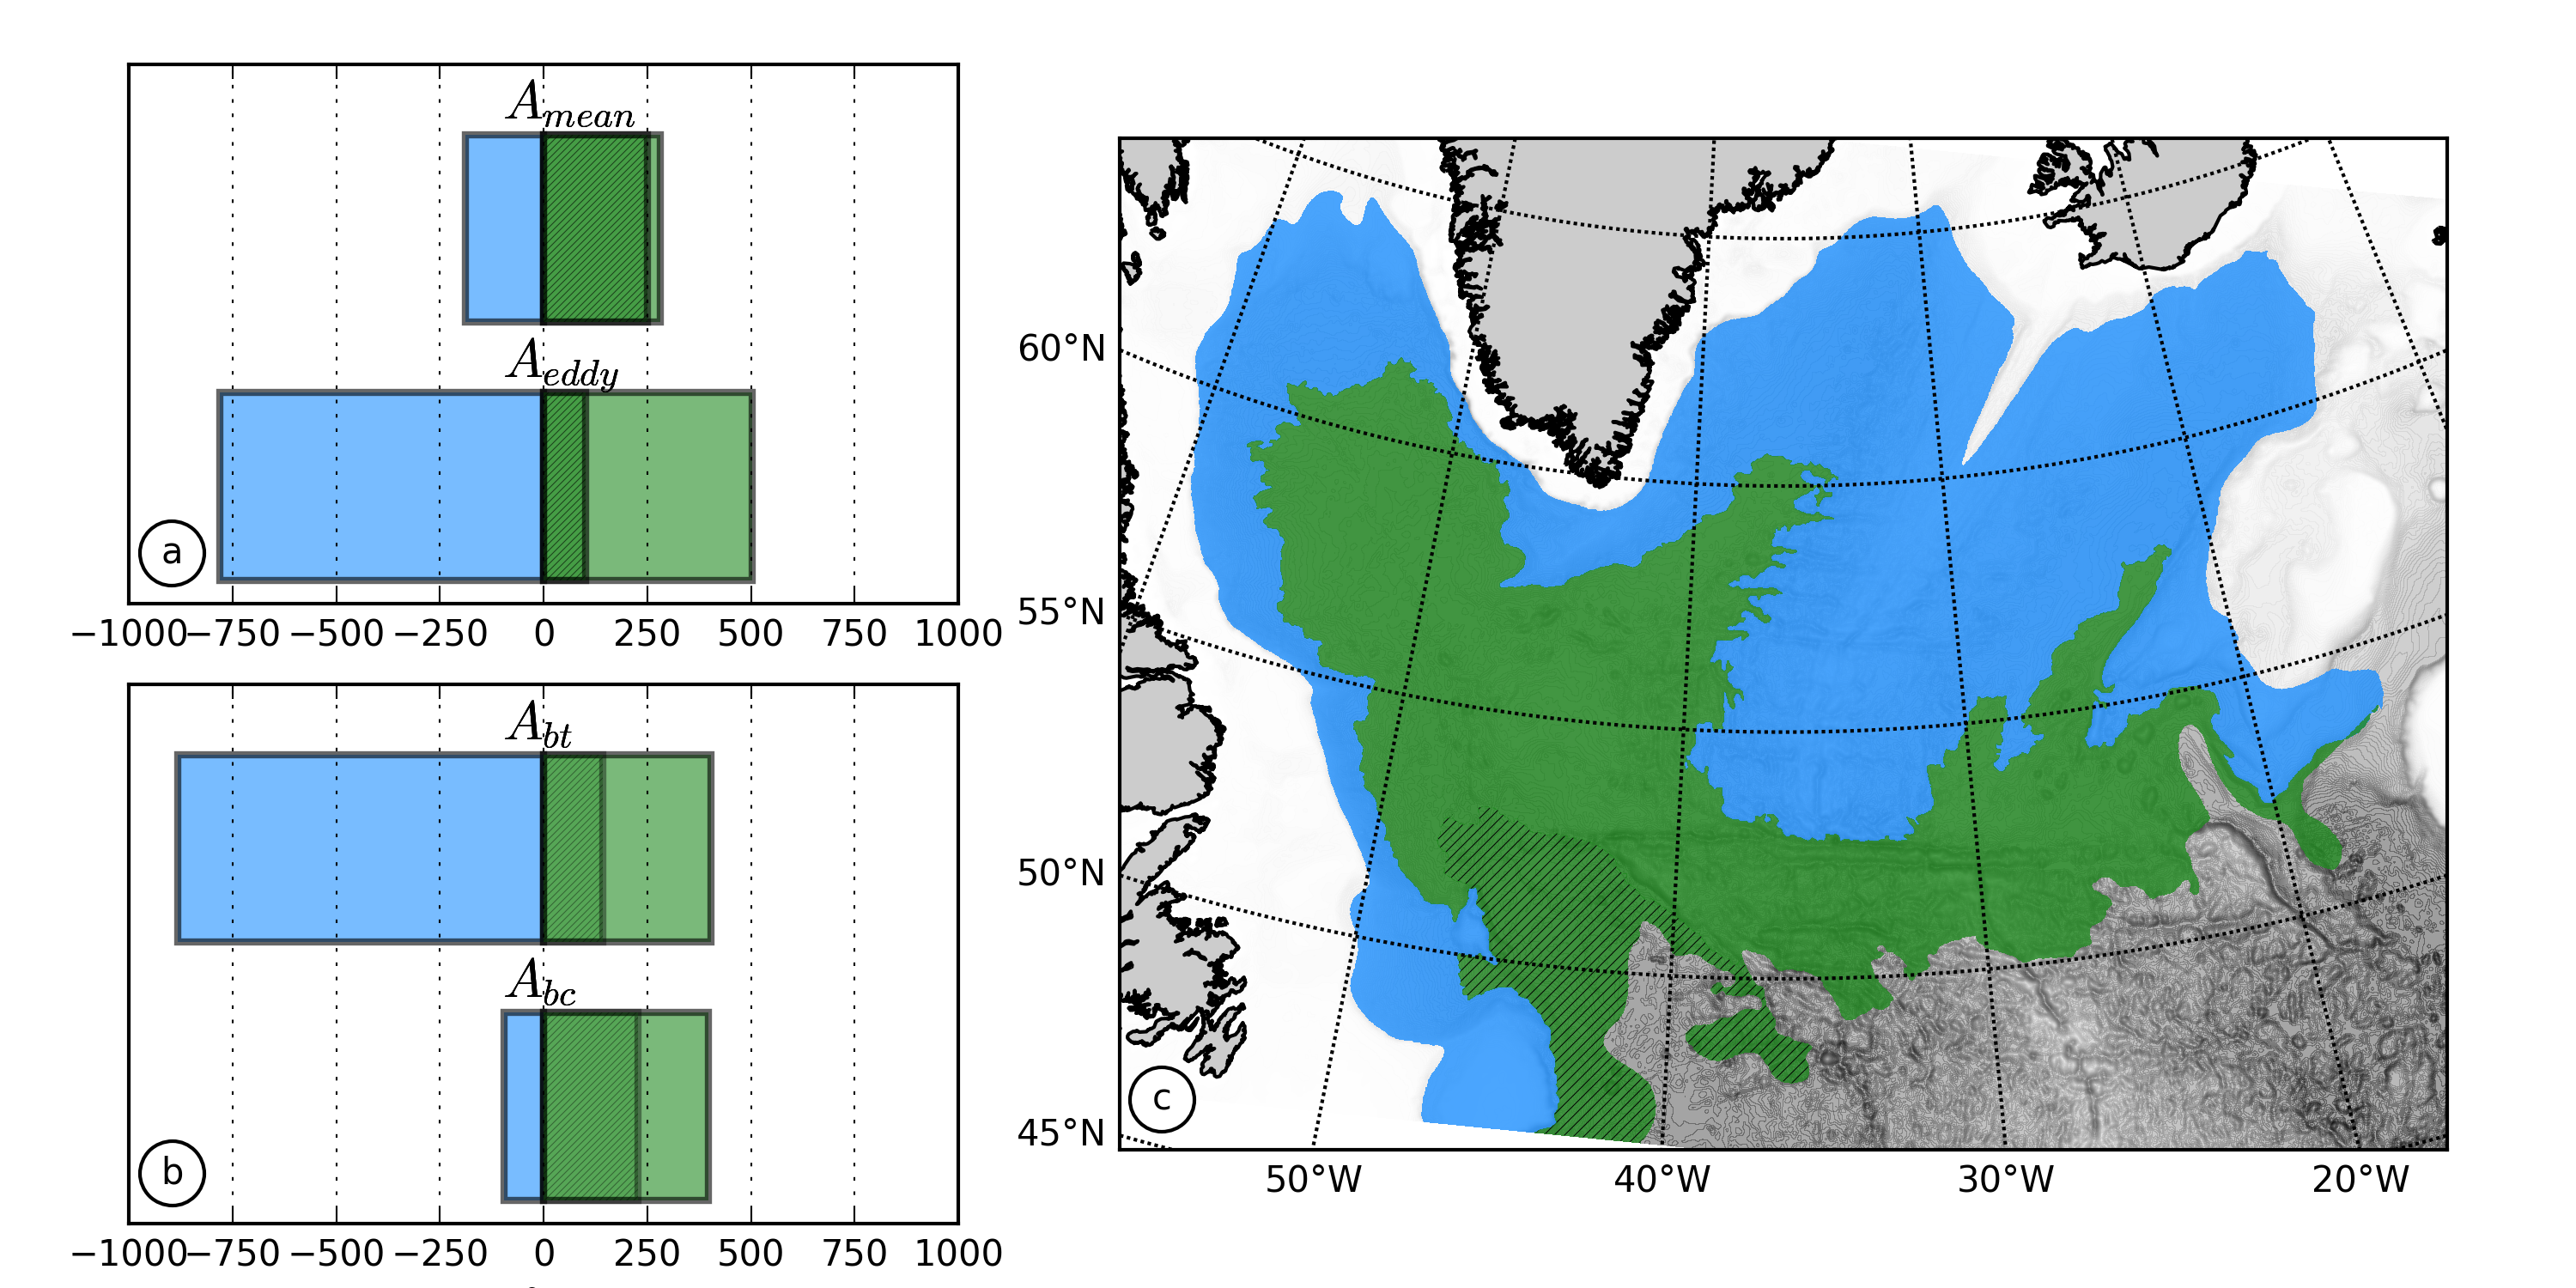
\includegraphics[width=15cm]{./v_b/int_NL_bound_in.png}}
\caption{Integration of the Non linear term in boundary and inner area for the -3 Sv contour for  the barotropic-baroclinic decomposition and the mean-eddy decomposition (left). A finer decomposition of the inner area separating the NWC (middle,blue) and the rest of the gyre (right,green).}
\label{int_NL}
\end{figure} 


It is also possible to decompose the NL term into a time mean and eddy part by writing $u = \langle u \rangle + u^*$ where $\langle \bullet\rangle$ is the time average and the star denotes the fluctuation part. By putting this in the non linear operator $A_{\Sigma}$ we have:


$$A_{\Sigma}(u,v)=\underbrace{A_{\Sigma}(\langle u \rangle, \langle v \rangle)}_{A_{\Sigma}^{mean}} + \underbrace{A_{\Sigma}(u^*,v^*)}_{A_{\Sigma}^{eddy}} +\underbrace{\langle  2\frac{\partial ^2 \overline{\langle v \rangle v^*} -\overline{\langle u \rangle u^*}}{\partial xy} +\frac{\partial ^2 \overline{\langle u \rangle v^*} + \overline{\langle v \rangle u^*}}{\partial xx} - \frac{\partial ^2 \overline{\langle u \rangle v^*} +\overline{ \langle v \rangle u^*}}{\partial yy}\rangle}_{\varepsilon}$$.


The $\varepsilon$ part is the residue of the cross product and its value is negligible compared to both the mean and eddy parts. When integrated over the boundary area, the eddy component dominates over the mean one. In the inner part, the supply of barotropic vorticity is mainly linked to the eddy component but the mean component is non negligible. More specifically most of the mean signal is coming from the NWC, this being consistent with the result from \citet{wang2017}. While the eddy part is dominant for the rest of the inner gyre.  %Taking into account that the NWC covers most of the need for the for the mean signal, the signal generated inside the boundary might be used for the shelf dynamics among other things. Also, vorticity advection by eddies generated along the boundary area is too large compared to what is needed by the interior (when excluding the NWC), the leftover is advecting barotropic vorticity outside of the domains. 


We can identify several processes for providing barotropic vorticity to the subpolar gyre. The most important is the eddy contribution coming from the boundary area that is associated with a barotropic contribution. Barotropic vorticity is also provided through a mean-baroclinic signal coming from the NWC. In comparison, in the lower resolution simulation (not shown) most of the vorticity is advected inside the gyre by mean-barotropic processes but the amplitude of the NL term is cut by half.

\subsection{Discussion}

In this part we studied the dynamics of the North Atlantic subpolar gyre using an eddy-resolving simulation ($\Delta x \approx$ 2 km) with terrain following coordinates allowing a good representation of flow-topography interactions. Our study agrees with previous works putting forward the importance of the topography through the Bottom Pressure Torque into driving the dynamics of the gyre along with the wind, corresponding to a topographic Sverdrup balance. But these previous studies were mostly made using low resolution simulations which is limiting the eddy activity in the area and tends to overestimate the dissipation by viscous terms near steep topography.

It is commonly admitted that non linear advective terms can be locally important for the dynamics of a particular area but tends to be negligible when integrated over a large domain. Here we showed the importance of this term into driving the interior dynamics of the subpolar gyre through a combination of mean and eddy effects. The major input of barotropic vorticity is due to barotropic eddy activity which redistributes the vorticity created along the topography by the bottom pressure torque. The second source is the North Atlantic Current by a mean baroclinic signal in the North West Corner.

We then emphasize that the role of the eddy activity in the North Atlantic Subpolar Gyre is essential if we want to reproduce correctly the dynamics of the gyre. The major source of eddies in this region is related to instability of the boundary currents. A good representation in models requires to resolve small scale processes that only high enough resolution simulations can solve.

\section{On the dynamics of the Rockall Trough anticyclone}
 
This section is a study made in collaboration with Angelina Smilenova, a PhD student at National University of Ireland, Galway (NUIG). Using co-analysis of altimetry, in-situ measurement she presents new insights on a persistent, non-stationary, deep anticyclonic vortex in the Rockall Trough (55$^{\circ}$ N, 12.5$^{\circ}$ W, west of Ireland) \citep{smilenova}. Similar deep quasi-permanent eddies can be found in other parts of the ocean. One well studied example is the Lofoten Vortex \citep{kohl,raj}. Dynamical studies of this feature have put forward the importance of smaller scale eddies for its formation and variability \cite{volkov15}. Our high resolution simulation is able to represent accurately the variability and the structure of the anticyclone. Here we investigate the dynamics of the RT anticcylone using our high resolution model.

\subsection{Eddy representation in the model}

The variability of the vortex can be evaluated trough the EAPE signal presented in figure \ref{energy}. In the RT, both model and observations show a local maximum with comparable amplitude northwest of Ireland, related to the presence of the RT anticyclone.

The mean vertical structure of the flow at this location is shown in Figure\ref{sec},b for the model along with in-situ  observations from Smilenova et al, 2019 \cite{smilenova}. Observations shown in Figure\ref{sec},a correspond to a transect done in January 2011. The observational velocity is derived from the temperature and salinity measurements assuming geostrophic balance.


\subsection{Barotropic vorticiy balance}

The RT anticyclone has a strong barotropic signature (Fig. \ref{sec}). An effective way to understand its dynamics is to look at the balance of barotropic vorticity. Such balance will provide information on the sources and sinks of anticyclonic vorticity and help us understand how the circulation can be sustained over such a long period. 


\begin{figure}[H]
\centerline{\includegraphics[width=15cm]{./fig_RT/section_RT_vit.png}}
\caption{(a) One-year mean of barotropic vorticity from the model. (b-c) Vertical sections of potential density (black contours) and cross-section velocity (colors) along the section shown in blue in panel a from in-situ observations in January 2011 (a) and from the model (b).}
\label{sec}
\end{figure}


If we take the equation presented in the previous section and integrate over a long enough period, the rate becomes negligible compared to the other terms, and the time-mean planetary vorticity advection reduces to $\left<-\nabla.(f\overline{u})\right>\approx \left<-\beta \overline{V}\right>$ as  $\left< \frac{\partial \eta }{\partial t} \right> \approx 0$.


The different terms of the barotropic vorticity balance are integrated over an area corresponding to the mean position of the vortex (Fig \ref{vort_balance}), defined as the -0.005 m.s$^{-1}$ barotropic velocity amplitude contour (Fig \ref{sec}). The main source for the anticyclonic circulation of the vortex is the non-linear term $A_{\Sigma}$. The main sinks of barotropic vorticity are the BPT and the Bottom Drag Curl (BDC). As a result of the small area covered by the eddy, the wind contribution is small, meaning that the wind stress does not contribute much to the vortex forcing.  

\subsection{Non-linear forcing of the RT anticyclone}


Using the same previous decomposition for the NL term we can study accurately which type of NL activity is feeding the RT vortex. The NL term is strongly dominated by its eddying part. The time-mean flow does not feed the RT anticyclone, and the vorticity is provided only by eddy vorticity fluxes. The decomposition into a barotropic and a baroclinic part also shows only one term being dominant:  the baroclinic component is much larger than the barotropic one. The main source of negative barotropic vorticity for the vortex is due to baroclinic eddy vorticity fluxes. 

\begin{figure}[H]
\centerline{\includegraphics[width=15cm]{./fig_RT/BV_int_RT.png}}
\caption{Integration of the Barotropic Vorticity balance over the RT anticyclone (left) and decompositions of the non-linear term between mean and eddy components, and between barotropic and baroclinic components (right)}
\label{vort_balance}
\end{figure} 

This vorticity balance can be interpreted as the RT vortex being fed by smaller subsurface anticyclonic eddies with a localized structure in the vertical. This is illustrated by a typical example of a smaller scale anticyclonic vortex merging with the RT anticyclone (Fig. \ref{fusion}). Snapshots of relative vorticity at 1000-m depth show the formation of a negative vorticity filament along the Porcupine bank (figure. \ref{fusion},a). The filament rolls up and form an anticyclonic eddy (figure. \ref{fusion},b), which is attracted by the RT anticyclone (figure. \ref{fusion},c), and is stretched around the RT anticyclone until they fully merge (figure. \ref{fusion},d). 

\begin{figure}[H]
\centerline{\includegraphics[width=15cm]{./fig_RT/snapshot_fusion_quiv.png}}
\caption{Sequence of snapshots of $\zeta/f$ at 1000-m depth showing the formation of a smaller eddy at Porcupine Bank later merging with the RT anticyclone. Frames are 6 days apart starting at the upper-left panel and proceed according to the labels }
\label{fusion}
\end{figure} 

\subsection{Eddy generation}
\medskip

The RT anticyclone seems to be fed mostly by small baroclinic anticyclonic eddies. In this section, we investigate the generation mechanisms for these smaller scale eddies.

Generation of anticyclonic eddies at this depth is mostly a result of current-topography interactions around the RT. Wintertime convection does not penetrate as deep.

The mean current is flowing cyclonically around the RT, i.e. with the shallower topography on his right. Frictional effects at the bottom will then trigger generation of negative relative vorticity and negative potential vorticity (PV) in the bottom boundary layer. When the boundary layer detaches from the slope, it can lead to centrifugal instability and formation of coherent vortices \cite{molemaker, gula16}.


The PV is defined by $q = \omega _a.\nabla b$, with $\omega _a = f\textbf{z}+\nabla \times \textbf{u}$ the absolute vorticity and the buoyancy gradient $b = -g\frac{\sigma}{\rho _0}$ where $\sigma$ is the potential density referenced to the surface, $\rho _0$ the mean reference density and $g$ the gravitational acceleration. The flux form of the PV equation can be written \cite{gula19}:

$$\frac{\partial q}{\partial t} + \nabla.[\underbrace{q\textbf{u}}_{J_A} - \underbrace{\omega _a\frac{D b}{D t}}_{J_D}+\underbrace{\nabla b \times \textbf{F}}_{J_F}] = 0$$

where \textbf{F} corresponds to the non conservative forces per unit mass. Each term respectively represent the PV advection, the diabatic flux and the frictional flux. When integrated between two isopycnal levels that intersect the seafloor but do not outcrop (hereafter I) the previous equation can be reduced to:

$$\frac{\partial}{\partial t} \int _I q dV= \int _I \underbrace{J_b}_{-(J_D+J_F)} dV$$,

meaning that the sources of potential vorticity along a slope are driven by diabatic and frictional effects. Thus, large values of the $J_b$ vector would indicate the most likely spots for a recurrent generation of eddies.

\begin{figure}[H]
\centerline{\includegraphics[width=15cm]{./fig_RT/Jbot_mean_quiv_2.png}}
\caption{Time mean PV flux at the bottom. The green contours correspond to the mean intersection of the 27.3,27.6 and 27.8 kg.m$^{-3}$ with the topography}
\label{pv_flux}
\end{figure}

The bottom PV fluxes are negative all around the RT (Fig. \ref{pv_flux}), in agreement with the orientation of the mean current flowing cyclonically around the RT. Hot spots are visible along the Porcupine bank and the Rockall Plateau. The strongest signals are located, on average, between the 27.3 and 27.6 kg.m$^{-3}$ isopycnals. The negative PV flux is dominated by frictional fluxes, the diabatic flux tends to generate positive input of PV (not shown). 


As the PV is conserved between two isopycnals, an eddy generated in a given density range will stay in this density range and move isopycnally inside the basin. Looking at the vertical structure of the vortex (Fig. \ref{sec}), we see that eddies generated along the topography between the 27.3 and 27.6 kg.m$^{-3}$, on average between 500 and 1000 m, will deepen when approaching the vortex and merge with it at the base of its core.


%%%%%%%%%%%%%%%%%%%%%%%%%%%%%%%%%%

\subsection{Lagrangian tracking of water masses}

We have identified the locations where anticyclonic vorticity is generated in the RT. To further investigate if the eddies generated along the slope can reach the RT anticyclone, we use a Lagrangian approach. 


We seed neutrally buoyant Lagrangian particles at the last time step of the simulation and advect them backward in time for one year. This allows us to track their trajectories and identify where particles are coming from. The vortex is separated in three density ranges: light (lighter than 27.3 kg.m$^{-3}$), intermediate (between 27.3 and 27.6 kg.m$^{-3}$) and heavy (higher than 27.6 kg.m$^{-3}$) waters. We compute the 2-D Probability Density Function (PDF) for the particles originating from each layer (Fig \ref{PDF}). The PDF is binned on a 1/5$^{\circ}$ grid and corresponds, for each bin, to the probability that a particle has been located inside this bin at least once during its lifetime \cite{vansebille}.

\begin{figure}[H]
\centerline{\includegraphics[width=15cm]{./fig_RT/PDF_RT.png}}
\caption{Probability that a particle occupies a particular bin at least once during the considered time span in different density ranges}
\label{PDF}
\end{figure}

Water lighter than 27.6 kg.m$^{-3}$ is mostly originating from the current flowing northward along the Porcupine Bank, where we observe a strong anticyclonic eddy generation.


\subsection{Discussion }

The dynamics of a deep, quasi-permanent, non-stationary anticyclone in the Rockall Trough has been studied in a succession of nested simulations ($\Delta$ x= 6 to 2 km).


The main source of negative vorticity for the vortex is due to eddy vorticity fluxes, mostly due to the merging of smaller anticyclonic eddies generated between 500 and 1000 m depth. This input of anticyclonic vorticity is balanced by topographic effects through the bottom pressure torque and the bottom drag curl acting as anticyclonic vorticity sinks. The intensification of the RT anticyclone implies a barotropization of its structure, which results in an intensification of the bottom currents. These currents are responsible for a positive drag curl and positive bottom pressure torque counter-acting the intensification of the RT vortex. 

Thanks to a combined study using the potential vorticity flux and a Lagrangian approach we were able to locate the main generation area for these eddies along the Porcupine bank. They are created predominantly between the 27.3 and 27.6 kg.m$^{-3}$ isopycnals and are reaching the RT anticyclone just below its core.

\section{Conclusion}

The role of topography in the subpolar gyre is investigated using a high resolution simulation ($\Delta X \approx$ 2 km)  with the terrain following model ROMS. At this resolution the mean flow characteristics and the mesoscale variability are in good agreement with the observations.   

A barotropic vorticity budget allowed us to confirm that the topography plays a key role in the subpolar gyre. Barotropic vorticity is generated along topography by the bottom pressure torque and advected toward the inside by barotropic eddy non-linear effects. The non linear term is the prevailing forcing driving the dynamics before the wind stress curl which greatly call into question the Sverdrup dynamics in this area.

Our simulation is also an interesting tools to study the mesoscale activity in the subpolar gyre. Indeed we found out it allows a greater diversity in the mesoscale processes that lower resolution simulations cannot solve. We took the opportunity to study the dynamics of a newly discovered quasi-permanent anticyclone in the Rockall Trough, west of Ireland. The results of our analysis showed that the vortex is mainly fed by smaller deep anticyclones generated along the Porcupine Bank and reaching the vortex at the base of its core. We have yet to properly identify what are the main processes generating the smaller anticyclones along the Porcupine Bank.


\section{Overview and Perspective}

The original aim of this Phd was to study the dynamics and to characterize processes driving the mixing in the vicinity of the Reykjanes Ridge. During the first part of the thesis I spent time working with the ROMS model to design a new set of simulations. I studied North-Atlantic scale simulations with different numerical and physical options to choose the most appropriate setup for our study. While working on the modelling of the subpolar gyre at higher resolution, many processes drew out our attention and raised several questions. This led us to reconsider our objectives and study the impact of the eddies and topography on the dynamics of the gyre, the higher resolution bringing new perspective on a wider range of processes that were better resolved. This also gave me the opportunity to collaborate with other projects studying mesoscale features in the gyre through observations. These different steps build a project that drifted from the original target but allowed me to take the time to develop new skills and to ripen new perspectives for future works.

The next couple of months will be of utmost importance in the finalization of this thesis. The objective of the next month is to finish the article in preparation on the dynamics of the subpolar gyre in an eddy resolving simulation, which is partially presented in section 4 of this report. The following months will be entirely dedicated to the writing of the manuscript. The first step will be to think of a way to organize the outline in order to fit all the elements together. The objective is to finish the manuscript before the end of September allowing a defense for November or December.


\newpage
\bibliographystyle{ametsoc2014}
\bibliography{biblio_rapp}

\end{document}
